\documentclass[]{report}
\voffset=-1.5cm
\oddsidemargin=0.0cm
\textwidth = 470pt
\usepackage[utf8]{inputenc}
\usepackage[english]{babel}
\usepackage{framed}

\usepackage{multicol}
\usepackage{amsmath}
\usepackage{amssymb}
\usepackage{enumerate}
\usepackage{multicol}

\begin{document}


%
%
%


\chapter{Session 1}

\section*{Part 1 : Binary numbers}
\subsection*{Question 1 }
Working in base 2 and showing all your workings, compute the following.
$(10110)_2 \times (111)_2$

\begin{itemize}
	\item Express the binary number $(1101.101)_2$ as a decimal, showing all your workings
	\item Express the decimal number $(3599)_{10}$ in base 2
\end{itemize}



\begin{itemize}
	%---------------------------%
	\item[(a)] Express the following binary numbers as decimal numbers
	\begin{itemize}
		\item[(i)] $11011$
		\item[(ii)] $100101$
	\end{itemize}
	%---------------------------%
	\item[(b)] Express the following decimal numbers as binary numbers
	\begin{itemize}
		\item[(i)] 6
		\item[(ii)] 15
		\item[(iii)] 37
	\end{itemize}
	%---------------------------%
	\item[(c)] Perform the following binary additions
	\begin{itemize}
		\item[(i)] $1011+ 1111$
		\item[(ii)] $10101  + 10011$
		\item[(iii)] $1010 + 11010$
	\end{itemize}
	%---------------------------%
	
\end{itemize}
% End of Subsection

\subsection*{Part 1b : Hexadecimal numbers}
%------------------------------------------------------------------------%
\begin{itemize}
	\item[(i)] Calculate the decimal equivalent of the hexadecimal number $(A2F.D)_{16}$
	\item[(ii)] Working in base 2, compute the following binary additions, showing all you workings
	\[(1110)_2 + (11011)_2 + (1101)_2 \]
	\item[(iv)] Express the recurring decimal $0.727272\ldots$ as a rational number in its simplest form.
\end{itemize}




\subsection*{Part E: Miscellaneous Questions}
\begin{itemize}
	\item[(i)] Given x is the irrational positive number $\sqrt{2}$, express $x^8$ in binary notation\\
	\item[(ii)] From part (i), is $x^8$ a rational number?
\end{itemize}
\newpage

%-----------------------------------------------------%
	\subsection*{Part A :  Binary numbers}
	\begin{itemize}
		%---------------------------%
		\item[(a)] Express the following binary numbers as decimal numbers
		\begin{itemize}
			\item[(i)] $11011$
			\item[(ii)] $100101$
		\end{itemize}
		%---------------------------%
		\item[(b)] Express the following decimal numbers as binary numbers
		\begin{itemize}
			\item[(i)] 6
			\item[(ii)] 15
			\item[(iii)] 37
		\end{itemize}
		%---------------------------%
		\item[(c)] Perform the following binary additions
		\begin{itemize}
			\item[(i)] $1011+ 1111$
			\item[(ii)] $10101  + 10011$
			\item[(iii)] $1010 + 11010$
		\end{itemize}
		
	\end{itemize}
	% End of Subsection
	
	\section*{Part A: Number Systems - Binary Numbers}
	\begin{enumerate}
		\item Express the following decimal numbers as binary numbers.
		\begin{multicols}{4}
			\begin{itemize}
				\item[i)] $(73)_{10}$
				\item[ii)] $(15)_{10}$
				\item[iii)] $(22)_{10}$
			\end{itemize}
		\end{multicols}
		
		All three answers are among the following options.
		\begin{multicols}{4}
			\begin{itemize}
				\item[a)] $(10110)_{2}$ %22
				\item[b)] $(1111)_{2}$ %15
				\item[c)] $(1001001)_{2}$ %73
				\item[d)] $(1000010)_{2}$ %64
			\end{itemize}
		\end{multicols}
		
		\item Express the following binary numbers as decimal numbers.
		\begin{multicols}{4}
			\begin{itemize}
				\item[a)] $(101010)_{2}$
				\item[b)] $(10101)_{2}$
				\item[c)] $(111010)_{2}$
				\item[d)] $(11010)_{2}$
			\end{itemize}
		\end{multicols}
		\item Express the following binary numbers as decimal numbers.
		\begin{multicols}{4}
			\begin{itemize}
				\item[a)] $(110.10101)_{2}$
				\item[b)] $(101.0111)_{2}$
				\item[c)] $(111.01)_{2}$
				\item[d)] $(110.1101)_{2}$
			\end{itemize}
		\end{multicols}
		\item Express the following decimal numbers as binary numbers.
		\begin{multicols}{4}
			\begin{itemize}
				\item[a)] $(27.4375)_{10}$  %
				\item[b)] $(5.625)_{10}$
				\item[c)] $(13.125)_{10}$
				\item[d)] $(11.1875)_{10}$
			\end{itemize}
		\end{multicols}
	\end{enumerate}
	\newpage
	\section*{Part B: Number Systems - Binary Arithmetic}
	%http://www.csgnetwork.com/binaddsubcalc.html
	%(See section 1.1.3 of the text)
	\begin{enumerate}
		\item Perform the following binary additions.
		\begin{multicols}{2}
			\begin{itemize}
				\item[a)] $(110101)_{2}$ + $(1010111)_{2}$
				\item[b)] $(1010101)_{2}$ + $(101010)_{2}$
				\item[c)] $(11001010)_{2}$ + $(10110101)_{2}$
				\item[d)] $(1011001)_{2}$ + $(111010)_{2}$
			\end{itemize}
		\end{multicols}
		
		\item Perform the following binary subtractions.
		\begin{multicols}{2}
			\begin{itemize}
				\item[a)] $(110101)_{2}$ - $(1010111)_{2}$
				\item[b)] $(1010101)_{2}$ - $(101010)_{2}$
				\item[c)] $(11001010)_{2}$ - $(10110101)_{2}$
				\item[d)] $(1011001)_{2}$ - $(111010)_{2}$
			\end{itemize}
		\end{multicols}
		
		
		\item Perform the following binary multiplications.
		\begin{multicols}{2}
			\begin{itemize}
				\item[a)] $(1001)_{2}\times( 1000)_{2}$  % 9 by 8
				\item[b)] $(101)_{2}\times(1101)_{2}$ % 5 by 11
				\item[c)] $(111)_{2}\times(1111)_{2}$ % 7 by 15
				\item[d)] $(10000)_{2}\times(11001)_{2}$    %16 by 25
			\end{itemize}
		\end{multicols}
		
		
		
		\item Perform the following binary multiplications.
		%\begin{multicols}{2}
		%\begin{itemize}
		%\item[a)] $(1001000)_{2} \div ( 1000)_{2}$
		%\item[b)] $(101101)_{2} \div (1001)_{2}$
		%\item[c)] $(1001011000)_{2} \div (101000)_{2}$
		%\item[d)] $(1100000)_{2} \div (10000)_{2}$
		%\end{itemize}
		%\end{multicols}
		
		\begin{enumerate}
			\item Which of the following binary numbers is the result of this binary division: $(10)_{2} \times ( 1101)_{2}$. % % (2) /  (13)
			\begin{multicols}{2}
				\begin{itemize}
					\item[a)] $(11010)_{2}$ %26
					\item[b)] $(11100)_{2}$ %28
					\item[c)] $(10101)_{2}$ %21
					\item[d)] $(11011)_2$ %27
				\end{itemize}
			\end{multicols}
			\item Which of the following binary numbers is the result of this binary division: $(101010)_{2} \times( 111 )_{2}$. % (4) /  (6)
			\begin{multicols}{2}
				\begin{itemize}
					\item[a)] $(11000)_{2}$ %24
					\item[b)] $(11001)_{2}$ %25
					\item[c)] $(10101)_{2}$ %21
					\item[d)] $(11011)_2$ %27
				\end{itemize}
			\end{multicols}
			\item Which of the following binary numbers is the result of this binary division: $(1001110)_{2}\times ( 1101 )_{2}$. % (9) /  (3)
			\begin{multicols}{2}
				\begin{itemize}
					\item[a)] $(11000)_{2}$ %24
					\item[b)] $(11001)_{2}$ %25
					\item[c)] $(10101)_{2}$ %21
					\item[d)] $(11011)_2$ %27
				\end{itemize}
			\end{multicols}
		\end{enumerate}
		
		%----------------------------------------------------------------%
		
		\item Perform the following binary divisions.
		%\begin{multicols}{2}
		%\begin{itemize}
		%\item[a)] $(1001000)_{2} \div ( 1000)_{2}$
		%\item[b)] $(101101)_{2} \div (1001)_{2}$
		%\item[c)] $(1001011000)_{2} \div (101000)_{2}$
		%\item[d)] $(1100000)_{2} \div (10000)_{2}$
		%\end{itemize}
		%\end{multicols}
		
		\begin{enumerate}
			\item Which of the following binary numbers is the result of this binary division: $(111001)_{2} \div ( 10011)_{2}$. % (57) /  (19)
			\begin{multicols}{2}
				\begin{itemize}
					\item[a)] $(10)_2$ %2
					\item[b)] $(11)_{2}$ %3
					\item[c)] $(100)_{2}$ %4
					\item[d)] $(101)_{2}$ %5
				\end{itemize}
			\end{multicols}
			\item Which of the following binary numbers is the result of this binary division: $(101010)_{2} \div ( 111 )_{2}$. % (42) /  (7)
			\begin{multicols}{2}
				\begin{itemize}
					\item[a)] $(11)_2$ %3
					\item[b)] $(100)_{2}$ %4
					\item[c)] $(101)_{2}$ %5
					\item[d)] $(110)_{2}$ %6
				\end{itemize}
			\end{multicols}
			\item Which of the following binary numbers is the result of this binary division: $(1001110)_{2} \div ( 1101 )_{2}$. % (78) /  (13)
			\begin{multicols}{2}
				\begin{itemize}
					
					\item[a)] $(100)_{2}$ %4
					\item[b)] $(110)_{2}$ %6
					\item[c)] $(111)_{2}$ %7
					\item[d)] $(1001)_2$ %9
				\end{itemize}
			\end{multicols}
		\end{enumerate}
		
		
	\end{enumerate}
	
	\newpage
	\section*{Part C: Number Bases - Hexadecimal}
	\begin{enumerate}
		
		\item Answer the following questions about the hexadecimal number systems
		\begin{itemize}
			\item[a)] How many characters are used in the hexadecimal system?
			\item[b)] What is highest hexadecimal number that can be written with two characters? \item[c)] What is the equivalent number in decimal form?
			\item[d)] What is the next highest hexadecimal number?
		\end{itemize}
		
		
		\item Which of the following are not valid hexadecimal numbers?
		\begin{multicols}{4}
			\begin{itemize}
				\item[a)] $73$
				\item[b)] $A5G$
				\item[c)] $11011$
				\item[d)] $EEF	$
			\end{itemize}
		\end{multicols}
		
		\item Express the following decimal numbers as a hexadecimal number.
		\begin{multicols}{4}
			\begin{itemize}
				\item[a)] $(73)_{10}$
				\item[b)] $(15)_{10}$
				\item[c)] $(22)_{10}$
				\item[d)] $(121)_{10}$
			\end{itemize}
		\end{multicols}
		
		
		\item Compute the following hexadecimal calculations.
		\begin{multicols}{4}
			\begin{itemize}
				\item[a)] $5D2+A30$
				\item[b)] $702+ABA$
				\item[c)] $101+111$
				\item[d)] $210+2A1$
			\end{itemize}
		\end{multicols}
	\end{enumerate}
	
	
	\newpage
	
	
	
	
	
	% \newpage
\section*{Part D : Base 5 and Base 8 numbers}
\begin{itemize}
	%---------------------------%
	\item[(a)] Suppose 2341 is a base-5 number
	Compute the equivalent in each of the following forms:
	\begin{itemize}
		\item[(i)] decimal number
		\item[(ii)] hexadecimal number
		\item[(iii)] binary number
	\end{itemize}
	%---------------------------%
	\item[(b)] Perform the following binary additions
	\begin{itemize}
		\item[(i)] $1011+ 1111$
		\item[(ii)] $10101  + 10011$
		\item[(iii)] $1010 + 11010$
	\end{itemize}
	%---------------------------%
\end{itemize}

	\subsection*{Part C : Base 5 and Base 8 numbers}
	\begin{itemize}
		%---------------------------%
		\item[(a)] Suppose 2341 is a base-5 number
		Compute the equivalent in each of the following forms:
		\begin{itemize}
			\item[(i)] decimal number
			\item[(ii)] hexadecimal number
			\item[(iii)] binary number
		\end{itemize}
		%---------------------------%
		
		%---------------------------%
	\end{itemize}
	\section*{Part E: Natural, Rational and Real Numbers}
	\begin{framed}
		\end{framed}
	
	\begin{enumerate}
		\item State which of the following sets the following numbers belong to. 
		\begin{multicols}{4}
			\begin{itemize}
				\item[1)] $18$
				\item[2)] $8.2347\ldots$
				\item[3)] $\pi$
				\item[4)] $1.33333\ldots$
				\item[5)] $17/4$
				\item[6)] $4.25$
				\item[7)] $\sqrt{\pi}$
				\item[8)] $\sqrt{25}$
				%\item[i)]
				%\item[j)] $(15)_{10}$
				%\item[k)] $\pi$
				%\item[l)] $11.132$
			\end{itemize}
		\end{multicols}
		\bigskip
		The possible answers are
		
		\begin{itemize}
			\item[a)] Natural number : $\mathbb{N} \subseteq \mathbb{Z } \subseteq \mathbb{Q} \subseteq \mathbb{R}$
			\item[b)] Integer : $ \mathbb{Z } \subseteq \mathbb{Q} \subseteq \mathbb{R}$
			\item[c)] Rational Number : $ \mathbb{Q} \subseteq \mathbb{R}$
			\item[d)] Real Number $\mathbb{R}$
			%\item[i)]
			%\item[j)] $(15)_{10}$
			%\item[k)] $\pi$
			%\item[l)] $11.132$
		\end{itemize}
		
	\end{enumerate}
	
		\begin{itemize}
			\item $\mathbb{N}$ : natural numbers (or positive integers) $\{1,2,3,\ldots\}$
			\item $\mathbb{Z}$ : integers $\{-3,-2,-1,0,1,2,3,\ldots\}$
			\begin{itemize}
				\item[$\ast$] (The letter $\mathbb{Z}$ comes from the word \emph{Zahlen} which means ``numbers" in German.)
			\end{itemize}
			\item $\mathbb{Q}$ : rational numbers
			\item $\mathbb{R}$ : real numbers
			\item $\mathbb{N} \subseteq \mathbb{Z } \subseteq \mathbb{Q} \subseteq \mathbb{R}$
			\begin{itemize}
				\item[$\ast$] (All natural numbers are integers. All integers are rational numbers. All rational numbers are real numbers.)
			\end{itemize}
					\end{itemize}
					
% \item The Fibonacci sequence $f_n$ is defined recursively by the rule
%   \begin{equation*}
%     \begin{cases}
%       f_0&=0\\
%       f_1&=1\\
%       f_n&=a_{n-1}+a_{n-2}
%     \end{cases}
%   \end{equation*}

%   \begin{enumerate}
%   \item
%     Write a program to evaluate the Fibonacci sequence and hence evaluate $f_{50}$.
%   \item
%     Let the sequence $g_n$ be defined as the ratio
%     \begin{equation*}
%       g_n = \frac{f_{n+1}}{f_n}
%     \end{equation*}
%     Write a program to evaluate the first $50$ terms of the sequence $g_n$.
%   \item
%     Assumming that the sequence $g_n$ has a limit $\phi$, find this limit.
%   \end{enumerate}



% \pagebreak
%   \begin{center}
%     \textbf{Assignment 1}
%     Due Tuesday Week 4 (Sept $28^th$)
%   \end{center}




\subsection*{Exercises Real and Rational Numbers}
\begin{itemize}
	\item[(i)] Express the recurring decimal $0.727272\ldots$ as a rational number in its simplest form.
\end{itemize}
%-------------------------------------------------------- %
\section*{Part F :  Scientific and Floating Point Notation}

\begin{itemize}
	\item Abscissa 
	\item Exponent (power)
\end{itemize}

With floating point notation, the abscisa must be between 0 and 1.
It is similar to scientific notation differing only by the fact that, with scientific notaiton, the abscissa is between 1 and 10.

\begin{itemize}
	\item Floating Point Notation
	\item $pi \approx 0.31415 \times 10^1$
	\item $pi \approx 3.1415 \times 10^0$
\end{itemize}
%-------------------------- %
%Section 2

%-----------------------------------------%



	\section*{Question 1}

	\subsection*{Part B :  Hexadecimal numbers}
	%------------------------------------------------------------------------%
	\begin{itemize}
		\item[(i)] Calculate the decimal equivalent of the hexadecimal number $(A2F.D)_{16}$
		\item[(ii)] Working in base 2, compute the following binary additions, showing all you workings
		\[(1110)_2 + (11011)_2 + (1101)_2 \]
		\item[(iv)] Express the recurring decimal $0.727272\ldots$ as a rational number in its simplest form.
	\end{itemize}
	
	

	\subsection*{Part D : Real and Rational Numbers}
	\begin{itemize}
		\item[(i)] Express the recurring decimal $0.727272\ldots$ as a rational number in its simplest form.
	\end{itemize}
	%-------------------------------------------------------- %
	\begin{itemize}
		\item[(i)] Given x is the irrational positive number $\sqrt{2}$, express $x^8$ in binary notation.
		\item[(ii)] From part (i), is $x^8$ a rational number?
	\end{itemize}
	
%----------------------------------------------------%
\subsection*{Binary and Hex}
\begin{itemize}
	\item[1A.1] Coverting from Binomial to Decimal
	\item[1A.2] Converting to Decimal
	\item[1A.3] Priority of Operation
	\item[1A.4] 
\end{itemize}

\subsection*{Numbers}
\begin{itemize}
	\item[1B.1] Real Numbers
	\item[1B.2] Rational Numbers
	\item[1B.3] Floating Point Aritmetic
	\item[1B.4] 
\end{itemize}
%================================================================ %

% %------------------------------------------------------
\section*{Part 1. Number Systems}

\subsection*{Section 1a. Binary Numbers}

\begin{enumerate}
	\item $1101001_{(2)}$
	\item $1101001_{(2)}$
	\item $1101001_{(2)}$
\end{enumerate}
%----------------------------------------- %
\section{Inequality Operators}
%------------------------------------------------------------------------- %

%\frametitle{Inequality Symbols}
\Large
Given $x = \sqrt{2}$ determine whether the following statements are true or false:

\begin{itemize}
	\item[(i)] $x \leq 2$
	\item[(ii)] $1.42 > x > 1.41$
	\item[(iii)] x is a rational number
	\item[(iv)] $\sqrt{2} = 2$
\end{itemize}

%------------------------------------------------------------------------- %
\section{Revision Questions}
	

	
	\[  2^ 4 = 2 \times 2 \times 2 \times 2 = 16 \]
	
	\[  5^ 3 = 5 \times 5 \times 5 =125 \]
	
	\subsubsection{Special Cases}
	
	Anything to the power of zero is always 1
	
	\[  X^ 0 = 1 \mbox{ for all values of X} \]
	
	Sometimes the power is a negative number.
	
	\[  X^{-Y} = { 1 \over X^Y}  \]
	
	Example 
	\[  2^{-3} = { 1 \over 2^3} = { 1 \over 8}  \]
	
	
	%====================================== %
	\newpage
	\begin{center}
		\huge{Mathematics for Computing}\\
		{\LARGE Session 2 : Set Theory}
	\end{center}
	
	
	% % \subfile{session02a.tex}

	%====================================== %
	\newpage
	\begin{center}
		\huge{Mathematics for Computing}\\
		{\LARGE Session 3 : Logic}
	\end{center}
	% %\subfile{session03a.tex}
	% % \subfile{session03d.tex}
	% % \subfile{DM0305DeMorgans.tex}
	
	%============================================ 
	\newpage
	\begin{center}
		\huge{Mathematics for Computing}\\
		\LARGE{Digraphs and Relations}
	\end{center}
	% % \subfile{session06a.tex}
	% % \subfile{session06e-antisymmetricrelations.tex}
	% % \subfile{session06f.tex}
	
	
	\subsubsection*{Question 1 : Binary numbers}
	\begin{itemize}
		%---------------------------%
		\item[(a)] Express the following binary numbers as decimal numbers
		\begin{multicols}{2}
			\begin{itemize}
				\item[(i)] $101$
				\item[(ii)] $1101$
				\item[(iii)] $11011$
				\item[(iv)] $100101$
			\end{itemize}
		\end{multicols}
		
		%---------------------------%
		\item[(b)] Express the following decimal numbers as binary numbers
		\begin{multicols}{2}
			\begin{itemize}
				\item[(i)] 6
				\item[(ii)] 15
				\item[(iii)] 37
				\item[(iv)] 77
			\end{itemize}
		\end{multicols}
		
	\end{itemize}
	%-------------%-------------%-------------%----------------
	\subsubsection*{Question 2}
	A number is expressed in base 5 as $(234)_5$. What is it as decimal number?
	Suppose you multiply $(234)_5$ by 5. what would be the answer in base 5.
	
	%-------------%-------------%-------------%----------------
	\subsubsection*{Question 3}
	
	Perform the following binary additions
	\begin{multicols}{2}
		\begin{itemize}
			\item[(i)] $1011+ 1111$
			\item[(ii)] $10101  + 10011$
			\item[(iii)] $1010 + 11010$
			\item[(iv)] $101010 + 10101 + 101$
		\end{itemize}
	\end{multicols}
	
	
	%-------------%-------------%-------------%----------------
	\subsubsection*{Question 4}
	Perform the binary additions
	
	\begin{itemize}
		\item $(10111)_2 +(111010)_2$
		
		\item $(1101)_2 + (1011)_2 + (1111)_2$
	\end{itemize}
	
	%-------------%-------------%-------------%----------------
	\subsubsection*{Question 5}
	
	Perform the binary subtractions using both the bit-borrowing method and the two's complement method.
	\begin{itemize}
		\item $(1001)_2 -(111)_2$
		\item $(110000)_2 -(10111)_2$
	\end{itemize}
	
	
	%-------------%-------------%-------------%----------------
	\subsubsection*{Question 6}
	
	Perform the binary multiplications
	\begin{itemize}
		\item $(1101)_2 \times (101)_2$
		\item $(1101)_2 \times (1101)_2$
	\end{itemize}
	
	
	%-------------%-------------%-------------%----------------
	\subsubsection*{Question 7}
	\begin{itemize}
		
		
		\item[(a)] What is highest Hexadecimal number that can be written with two characters, and what is it's equivalent in decimal form?
		What is the next highest hexadecimal number?
		
		% \[FF = 255\] % Remark 
		\item[(b)] Which of the following are not valid hexadecimal numbers?
		
		\begin{multicols}{2}
			\begin{itemize}
				\item[(i)] A5G 	
				\item[(ii)] 73 
				\item[(iii)] EEF	
				\item[(iv)] 101
			\end{itemize}
		\end{multicols}
	\end{itemize}	
	
	
	
	%-------------%-------------%-------------%----------------
	\subsubsection*{Question 8 : Binary Substraction}
	\textbf{Exercises:}
	
	\begin{multicols}{2}
		\begin{itemize}
			\item[(i)] 110 - 10	
			\item[(ii)] 101 - 11  
			\item[(iii)] 1001 - 11	
			\item[(iv)] 10001 - 100 
			\item[(v)] 101001 - 1101
			\item[(vi)] 11010101-1101
		\end{itemize}
	\end{multicols}
	
	
	
	%-------------%-------------%-------------%----------------
	\subsubsection*{Question 9}
	
	\begin{itemize}
		%---------------------------%
		\item[(a)] Suppose 2341 is a base-5 number
		Compute the equivalent in each of the following forms:
		\begin{itemize}
			\item[(i)] decimal number
			\item[(ii)] hexadecimal number
			\item[(iii)] binary number
		\end{itemize}
		%---------------------------%
		\item[(b)] Perform the following binary additions
		\begin{itemize}
			\item[(i)] $1011+ 1111$
			\item[(ii)] $10101  + 10011$
			\item[(iii)] $1010 + 11010$
		\end{itemize}
		%---------------------------%
	\end{itemize}
	
	%-------------%-------------%-------------%----------------
	\subsubsection*{Question 10}
	
	Calculate working in hexadecimal
	\begin{itemize}
		\item[(i)] $(BBB)_{16} + (A56)_{16}$
		\item[(ii)] $(BBB)_{16} - (A56)_{16}$
	\end{itemize} 
	
	
	%-------------%-------------%-------------%----------------
	\subsubsection*{Question 11}
	
	Write the hex number $(EC4)_{16}$ in binary.
	Write the binary number $(11110110101|)_2$ in hex.
	%-------------%-------------%-------------%----------------
	%-------------%-------------%-------------%----------------
	\subsubsection*{Question 12}
	
	Express the decimal number 753 in binary , base 5 and hexadecimal.
	
	%-------------%-------------%-------------%----------------
	%-------------%-------------%-------------%----------------
	\subsubsection*{Question 13}
	
	Express 42900 as a product of its prime factors, using index notation for repeated factors.
	
	%-------------%-------------%-------------%----------------
	%-------------%-------------%-------------%----------------
	\subsubsection*{Question 14}
	
	Expresse the recuring decimals 
	\begin{itemize}
		\item[(i)] $0.727272\ldots$
		\item[(ii)] $0.126126126....$
		\item[(iii)] $0.7545454545...$
	\end{itemize} 
	as rational numbers in its simplest form.
	
	%-------------%-------------%-------------%----------------
	%-------------%-------------%-------------%----------------
	\subsubsection*{Question 15}
	Given that $\pi$ is an irrational number, can you say whether $\frac{\pi}{2}$ is rational or irrational.
	or is it impossible to tell?
	
	%-------------------------------------------------------- %
	\subsubsection*{Question 16}
	\begin{itemize}
		\item[(i)] Given x is the irrational positive number $\sqrt{2}$, express $x^8$ in binary notation\\
		\item[(ii)] From part (i), is $x^8$ a rational number?
	\end{itemize}
	
	%-------------%-------------%-------------%----------------
	%-------------%-------------%-------------%----------------
	\subsubsection*{Question 17}
	\begin{enumerate}
		\item[(i)] 5/7 lies between 0.714 and 0.715.
		\item[(ii)] $\sqrt(2)$ is at least 1.41.
		\item[(iii)] $\sqrt(3)$  9s at lrast 1.732 and at most 1.7322.
	\end{enumerate}
	
	
	%-------------%-------------%-------------%----------------
	%-------------%-------------%-------------%----------------
	\subsubsection*{Question 18}
	\begin{itemize}
		\item[(i)] Write down the numbers 0.0000526 in floating point form.
		\item[(ii)] How is the number 1 expressed in floating point form.
	\end{itemize}
	
	
	%-------------%-------------%-------------%----------------
	%-------------%-------------%-------------%----------------
	\subsubsection*{Question 19}
	\begin{itemize}
		\item Deduce that every composite integer $n$ has a prime factor such that $p \leq \sqrt{n}$.
		\item Decide whether 899 is a prime.
	\end{itemize}
	
	%-------------%-------------%-------------%----------------
	%-------------%-------------%-------------%----------------
	\subsubsection*{Question 20}
	
	\begin{itemize}
		\item What would be the maximum numbber of digits that a decimal fraction with denominator 13 
		could have in a recurring block in theory?
		
		\item Can you predict which other fractions with denominator 13 will have the same digits as 1/13 in their recurring block?
	\end{itemize}
	
	
	
	%----------------------------------------- %
\section{Video 6}

%\frametitle{Inequality Symbols}
\Large
Convert the following statements into symbols:

\begin{itemize}
	\item $\sqrt{2}$ is less than 1.5 and greater than 1.4
	\item $\sqrt{2}$ is greater than or equal to 5
\end{itemize}



%------------------------------------------------------------------------- %
% Floating Point Notation
\chapter{Session 2}
% Ex 1
%--------------------------------- %
\section*{The Universal Set and the Empty Set}
\begin{itemize}
	\item The first is the \textbf{\textit{universal set}}, typically denoted $U$. This set is all of the elements that we may choose from. This set may be different from one setting to the next. 
	
	\item For example one universal set may be the set of all real numbers, denoted $\mathbb{R}$, whereas for another problem the universal set may be the whole numbers $\{0, 1, 2,\ldots\}$.
	
	\item The other set that requires consideration is called the \textit{\textbf{empty set}}. The empty set is the unique set is the set with no elements. We write this as $\{ \}$ and denote this set by $\emptyset$.
\end{itemize}
%---------------------------------%
\section*{Number Sets}
The font that the following symbols are written in (i.e. $\mathbb{N}$, $\mathbb{R}$) is known as \textit{\textbf{blackboard font}}.
\begin{itemize}
	\item $\mathbb{N}$ Natural Numbers ($1,2,3,\ldots$) 
	%	\textit{(Not used in the CIS102 Syllabus)}
	\item $\mathbb{Z}$ Integers ($-3,-2,-1,0,1,2,3, \ldots$)
	\begin{itemize}
		\item[$\bullet$] $\mathbb{Z}^{+}$ Positive Integers
		\item[$\bullet$] $\mathbb{Z}^{-}$ Negative Integers
		\item[$\bullet$] 0 is not considered as either positive or negative.
	\end{itemize}
	\item $\mathbb{Q}$ Rational Numbers
	\item $\mathbb{R}$ Real Numbers
	\item $\mathbb{C}$ Complex Numbers
\end{itemize}
%========================================================================================= %
\newpage
\section*{Rules of Inclusion, Listing and Cardinality}
For each of the following sets, a set is specified by the rules of inclusion method and listing method respectively. Also stated is the cardinality of that data set.
\subsection*{Worked example 1}
\begin{itemize}
	\item $\{ x : x $ is an odd integer $ 5 \leq x \leq 17 \}$
	\item $x = \{5,7,9,11,13,15,17\}$
	\item The cardinality of set $x$ is 7.
\end{itemize}

\subsection*{Worked example 2}
\begin{itemize}
	\item $\{ y : y $ is an even integer $ 6 \leq y < 18 \}$
	\item $y = \{6,8,10,12,14,16\}$
	\item The cardinality of set $y$ is 6.
\end{itemize}

\subsection*{Worked example 3}
A perfect square is a number that has a integer value as a
square root. 4 and 9 are perfect squares ($\sqrt{4} = 2$,
$\sqrt{9} = 3$).
\begin{itemize}
	\item $\{ z : z $ is an perfect square $ 1 < z < 100 \}$
	\item $z = \{4,9,16,25,36,49,64,81\}$
	\item The cardinality of set $z$ is 8.
\end{itemize}

\newpage

\subsection*{Exercises}
For each of the following sets, write out the set using the listing method.
Also write down the cardinality of each set.

\begin{itemize} 
	\item $\{ s : s $ is an negative integer $ -10 \leq s \leq 0 \}$
	\item $\{ t : t $ is an even number $ 1 \leq t \leq 20 \}$
	\item $\{ u : u $ is a prime number $ 1 \leq u \leq 20 \}$
	\item $\{ v : v $ is a multiple of 3 $ 1 \leq v \leq 20 \}$
\end{itemize}
%-------------------------------------------------% 
\newpage
\section*{Power Sets}
\subsection*{Worked Example}
Consider the set $Z$:
\[ Z = \{ a,b,c\}  \]
\begin{itemize}
	\item[(i)] How many sets are in the power set of $Z$? 
	\item[(ii)] Write out the power set of $Z$. 
	\item[(iii)] How many elements are in each element set?
\end{itemize}
%----------------------------------------------%
\subsection*{Solutions to Worked Example}

\begin{itemize}
	
	
	\item[(i)] There are 3 elements in $Z$. So there is $2^3 = 8$ element sets contained in the power set.
	
	\item[(ii)] Write out the power set of $Z$.
	\[ \mathcal{P}(Z) = \{ \emptyset, \{a\}, \{b\}, \{c\}, \{a,b\}, \{a,c\}, \{b,c\}, \{a,b,c\} \} \]
	
	\item[(iii)]
	\begin{itemize}
		\item[$\bullet$] One element set is the null set - i.e. containing no
		elements \item[$\bullet$] Three element sets have only elements \item[$\bullet$]
		Three element sets have two elements \item[$\bullet$] One element set
		contains all three elements \item[$\bullet$] 1+3+3+1=8
	\end{itemize}
\end{itemize}
\subsection*{Exercise}
For the set $Y = \{u,v,w,x\}$ , answer the questions from the
previous exercise


%------------------------------------------------------%

\section*{Complement of a Set}
%(2.3.1) 
Consider the universal set $U$ such that
\[U=\{2,4,6,8,10,12,15\} \]
For each of the sets $A$,$B$,$C$ and $D$, specify the complement sets.
{
	\LARGE
	\begin{center}
		\begin{tabular}{|c|c|}
			\hline
			Set &\phantom{sp} Complement \phantom{sp}\\
			\hline \phantom{sp} $A=\{4,6,12,15\}$ \phantom{sp} &
			$A^{\prime}=\{2,8,10\}$ \\ \hline $B=\{4,8,10,15\}$ & \\ \hline
			$C=\{2,6,12,15\}$ & \\ \hline $D=\{8,10,15\}$ & \\ \hline
			
		\end{tabular}
	\end{center}
}
%-------------------------------------%
% Binary Operations on Sets (2.3.2)
% Union , Intersection, Symmetric Difference
% Set Difference

%======================================================================================= %
\newpage
\section*{Set Operations}
\begin{itemize}
	\item Union ($\cup$) - also known as the \textbf{OR} operator. A union signifies a bringing together. The union of the sets A and B consists of the elements that are in either A or B.
	\item Intersection ($\cap$) - also known as the \textbf{AND} operator. An intersection is where two things meet. The intersection of the sets A and B consists of the elements that in both A and B.
	\item Complement ($A^{\prime}$ or $A^{c}$) - The complement of the set A consists of all of the elements in the universal set that are not elements of A.
\end{itemize}

\subsection*{Exercise}
Consider the universal set $U$ such that
\[U=\{1,2,3,4,5,6,7,8,9\} \] 
and the sets
\[A=\{2,5,7,9\} \] 
\[B=\{2,4,6,8,9\} \]

\begin{multicols}{2}
	\begin{itemize}
		\item[(a)] $A-B$
		\item[(b)] $A \otimes B$
		\item[(c)] $A \cap B$
		\item[(d)] $A \cup B$
		\item[(e)] $A^{\prime} \cap B^{\prime}$
		\item[(f)] $A^{\prime} \cup B^{\prime}$
	\end{itemize}
\end{multicols}

%======================================================================================= %
\newpage

\section*{Venn Diagrams}

Draw a Venn Diagram to represent the universal set
$\mathcal{U} = \{0,1,2,3,4,5,6\}$ with subsets:\\
$A = \{2,4,5\}$\\
$B = \{1,4,5,6\}$\\

\noindent Find each of the following
\begin{itemize}
	\item[(a)] $A \cup B $
	\item[(b)] $A \cap B $
	\item[(c)] $A-B$
	\item[(d)] $B-A$
	\item[(e)] $A \otimes B$
\end{itemize}
\newpage



%------------------------------------------------------------------------%
\begin{itemize}
	\item[(i)] Describe the following set by the listing method
	\[ \{ 2r+1 : r \in Z^{+} and r \leq 5  \} \]
	\item[(ii)] Let A,B be subsets of the universal set U.
	
	
\end{itemize}

%===================================================================================== %
\subsection*{Question 1}

\begin{itemize}
	\item $\{ s :  \mbox{ s is an odd integer and } 2 \leq s \leq 10 \}$
	\item $\{ 2m :  m \in Z \mbox{ and }5 \leq m \leq 10 \}$
	\item $\{ 2^t :  t \in Z \mbox{ and } 0 \leq t \leq 5 \}$
\end{itemize}

%=======================+============================================================== %
\subsection*{Question 2}

\begin{itemize}
	\item $\{12,13,14,15,16,17\}$
	\item $\{0,5,-5,10,-10,15,-15,.....\}$
	\item $\{6,8,10,12,14,16,18\}$
\end{itemize}

\subsection*{Question 7 : Membership Tables}
Using membership tables
\begin{tabular}{|ccc|c|c|c|}
	\hline
	% after \\: \hline or \cline{col1-col2} \cline{col3-col4} ...
	A & B & C & x & y & z \\\hline
	0 & 0 & 0 & 1 & 1 & 1 \\
	0 & 0 & 1 & 0 & 0 & 1 \\
	0 & 1 & 0 & 0 & 0 & 1 \\
	0 & 1 & 1 & 0 & 0 & 1 \\
	1 & 0 & 0 & 1 & 0 & 1 \\
	1 & 0 & 1 & 1 & 0 & 1 \\
	1 & 1 & 0 & 0 & 0 & 1 \\
	1 & 1 & 1 & 1 & 0 & 1 \\
	\hline
\end{tabular}
\begin{itemize}
	\item[(i)] Draw a venn diagram to show three subsets A,B and C of a universal set U intersecting in
	the most general way?
	\item[(ii)] How are sets $X$ and $Z$ related?
	\item[(iii)] Can you describe each of the subsets X,Y and Z in terms  of the
	sets A,B,C using the operations union intersection and set complement.
\end{itemize}
%================================================================ %


\subsection{Ellipsis}

When using Ellipsis, it should be clear what the pattern is

%-------------------------------------%


%-----------Reference to section 2.2.3 Power Sets




%-------------------------------------%

%----(Reference to Section 2.2.2 Cardinality)



%-------------------------------------% % Complement of a set


%--------------------------------------%
\subsection*{ Three Sets }

%- Section 2.3.5 %- Associative Law %- Distribution Law





%-------------------------------------% %- Section 3
Propositional Logic A statement is a declarative sentence that
is either true or false.
\begin{itemize}
	\item $\tilde q$ not q \item $p \vee q$ \item $p \wedge \tilde
	q$
\end{itemize}



%======================================================================================= %

Question 5


Let A, B be subsets of the universal set $\mathcal{U}$.

Use membership tables to prove De Morgan's Laws.


%
%Construct Membership tables for each of the sets
%(A-B) - C
%A-(B- C)
%
%(A-B) -C = A-(B-C)
%A
%


\begin{itemize}
	\item[a.] (1 mark) Write out the sample space for the outcomes for both players A and B.
	\item[b.] (1 mark) Write out the sample space for the outcomes of C, where C is the difference of the two scores (i.e. B-A)
	\item[c.] (1 mark) Are the sample points for the sample space of C equally probable? Provide a brief justification for your answer.
\end{itemize}

%----------------------------------------------------------%
\newpage
\section*{Section B: Set Operations}
\begin{itemize}
	\item[B.1] complement of A $A^{\prime}$
	\item[B.2] Union $A \cup B$
	\item[B.3] Intersection $A \cap B$
	\item[B.4] Relative Difference $A \otimes B$
	\item[A.5]
	\item[A.6]
	\item[A.7]
	\item[A.8]
\end{itemize}
\newpage


\begin{itemize}
	\item Specifying Sets
	\item Listing Method
	\item Rules of Inclusion method
\end{itemize}


\begin{itemize}
	\item Subsets Notation of a subset
	\item Cardinality of a set
	\item Power of a set
\end{itemize}

\subsection*{Operation on Sets}

\begin{itemize}
	\item The complement of Set
	\item Binary Operations
	\begin{itemize}
		\item Union
		\item Intersection
	\end{itemize}
	\item Membership tables
	\item Laws for Combining Sets
\end{itemize}

\newpage


\subsection*{Associative Laws}
\[ (A \cup B) \cup C =  A \cup (B \cup C)  \]
\[ (A \cap B) \cap C =  A \cap (B \cap C)  \]

\subsection*{Distributive Laws}
\[ (A \cup B) \cap C =  (A \cup B) \cap (A \cup C)  \]
\[ (A \cap B) \cup C =  (A \cap B) \cup (A \cap C)  \]


\[ (A \cup B) \cap B^{\prime} \]
%----------------------------------------------------------%
\section*{Section C: Real and Rational Numbers}

%----------------------------------------------------------%
\newpage
\section*{Formulae}
\begin{itemize}
	
	
	
	
	\item Bayes' Theorem:
	\begin{equation*}
	P(B|A)=\frac{P\left(A|B\right) \times P(B) }{P\left( A\right) }.
	\end{equation*}
	
	
	
	\item Binomial probability distribution:
	\begin{equation*}
	P(X = k) = ^{n}C_{k} \times p^{k} \times \left( 1-p\right) ^{n-k}\qquad \left( \text{where}\qquad
	^{n}C_{k} =\frac{n!}{k!\left(n-k\right) !}. \right)
	\end{equation*}
	
	\item Poisson probability distribution:
	\begin{equation*}
	P(X = k) =\frac{m^{k}\mathrm{e}^{-m}}{k!}.
	\end{equation*}
\end{itemize}

\section{Video 1 :  Set Theory Listing Method}
%--------------------------------------------%

%\frametitle{Set Theory : Listing Method}
\Large
Describe the following sets using the Listing Method

\begin{itemize}
	\item[(i)] $ \{ 10^m : -2 \leq m \leq 4, m \in \mathbb{Z} \} $
	\item[(ii)]  $ \{ \frac{1}{n}: 1 < n < 4, n \in \mathbb{Z} \} $
\end{itemize}


%--------------------------------------------%

%\frametitle{Set Theory : Listing Method}
\Large
\vspace{-4cm}
\textbf{Part 1:} $ \{ 10^m : -2 \leq m \leq 4, m \in \mathbb{Z} \} $


%--------------------------------------------%

%\frametitle{Set Theory : Listing Method}
\Large
\vspace{-4cm}
\textbf{Part 2:} $ \{ \frac{1}{n}: 1 < n < 4, n \in \mathbb{Z} \} $


% Ex 2
\section{Video 2 : Set Theory}
%--------------------------------------------%

%\frametitle{Set Theory : Set Operations}
\Large
Given the following sets

\begin{center}
	\begin{tabular}{|c|c|} \hline
		$\mathcal{U}$ & $\{1,2,3,4,5,6,7,8,9\}$ \\ \hline
		$\mathcal{A}$ & $\{1,2,5,6,8\}$ \\ \hline
		$\mathcal{B}$ & $\{3,5,7,8\}$ \\ \hline
		$\mathcal{C}$ & $\{5,6,7,8,9\}$ \\ \hline
	\end{tabular}
\end{center}

List the elements of the following
$A^{\prime} \cap B $\\
$A^{\prime} \cap C $\\

%--------------------------------------------%

\section*{Venn Diagrams}

Subsets of the universal set $\mathcal{U}$, intersecting in the most general way (Essentially this means - the venn diagram allows for all possible combinations of overlap.)

\begin{center}
	\begin{tabular}{|c|c|}
		\hline  &  \\ 
		\hline  &  \\ 
		\hline 
	\end{tabular} 
\end{center}

%-------------------------- %
%-------------------------- %
%Section 3

	\section*{Question 2}
	HibCollWorkSheet2
	
	%Listing Method
	%Rules of Inclusion
	%Cardinality
	%Venn diagrams
	
	$\in$
	$\subset$
	
	univeral Set $\mathcal{U}$
	Laws for Binary Operations
	Membership Tables
	
	De Morgan's Law
	
	
	\[A^{\prime} \cup B^{\prime} = A \cap B\]
	
	\subsection*{Part A : Builder Method}
	The following sets have been defined using the \textbf{Building Method} of notation. Re-write them by listing \textbf{some} of the elements.
	\begin{enumerate}
		\item $\{p | p$ is a capital city, p is in Europe$\}$
		\item $\{x | x = 2n - 5,$ x and n are natural numbers$\}$
		\item $\{y | 2y^2 = 50,$ y is an integer$\}$
		\item $\{z | z = n^3,$ z and n are natural numbers$\}$
	\end{enumerate}
	\subsection*{Part B : Sets}
	U = {natural numbers}; $A = \{2, 4, 6, 8, 10\}$; $B = \{1, 3, 6, 7, 8\}$. State whether each of the following is true or false:
	\begin{itemize}
		\item[(i)] $A \subset U$
		\item[(ii)] $B \subseteq A$
		\item[(iii)] $\emptyset \subset U$
	\end{itemize}
	
	%-------------------------------------- %
	
	\section*{Question 2}
	\subsection*{Part A : Builder Method}
	The following sets have been defined using the \textbf{Building Method} of notation. Re-write them by listing \textbf{some} of the elements.
	\begin{enumerate}
		\item $\{p | p$ is a capital city, p is in Europe$\}$
		\item $\{x | x = 2n - 5,$ x and n are natural numbers$\}$
		\item $\{y | 2y^2 = 50,$ y is an integer$\}$
		\item $\{z | z = n^3,$ z and n are natural numbers$\}$
	\end{enumerate}
	\subsection*{Part B : Sets}
	U = {natural numbers}; $A = \{2, 4, 6, 8, 10\}$; $B = \{1, 3, 6, 7, 8\}$. State whether each of the following is true or false:
	\begin{itemize}
		\item[(i)] $A \subset U$
		\item[(ii)] $B \subseteq A$
		\item[(iii)] $\emptyset \subset U$
	\end{itemize}
	
	%-------------------------------------- %
	
	
	\section*{Question 2}
	Describe the following set by the rules of inclusion method.
	
	Describe the following set by the listing method
	the set of positive multiples of 3 which are less than 20.
	
	Let A and B be subsets of univerisal set U
	
	Use the membership rule to prove that
	
	\[(A^\prime  \cap B)^\prime = A \cup B^\prime\]
	
	shade the region corresponding to this set on a Venn Diagram
	
	Given the universal set $\mathcal{U} = {1,2,3,4,5,6,7,8,9}$
	and the subsets $A=\{1,3,5,7\}$
	$B = \{6,7,8,9\}$
	list the set $A^\prime \cap B)^\prime$ 
	
	
	\Large
\begin{itemize}
	\item[(i)] $\{5,8\}$
	\item[(ii)] $\{1,2,3,4,5,6,7,8,9\}$ 
\end{itemize}


%Exercise 3
\section{Set Theory}
%--------------------------------------------%

%\frametitle{Set Theory : Set Operations}
\Large
\begin{itemize}
	\item[\textbf{A}] $ \{ 2n : n \in \mathbb{Z^{+}} \} $
	\item[\textbf{B}] $ \{ 3,6,9,12,15,18,\ldots \} $
\end{itemize}
\textbf{Questions}
\begin{itemize}
	\item[(i)] \textbf{A} is described by the rules of inclusion. Describe \textbf{A} with the listing method.
	\item[(ii)] \textbf{B} is described by the listing method. Describe \textbf{B} with the rules of inclusion. 
\end{itemize}




%------------------------------------%
\section*{Question 4}
\[ \mbox{Log}_4 64 + \mbox{Log}_5 625 + \mbox{Log}_9 3 \] 


%------------------------------------%
\section*{Question 5}
\begin{enumerate}
	\item Draw two non-isomorphic graphs with the following degree sequence.
	\[ 4,3,3,2,2,2,2,1,1\]
	\item
\end{enumerate}
%------------------------------------%

\section*{Question 7b}

Compute the following summation

\[ \sum^{i=100}_{i=25} i^2 + 3i -5)\]


%------------------------------------%

\section*{Section 2. Set Theory}

\begin{enumerate}
	\item
	\item
	\item
\end{enumerate}
\subsection*{Membership Tables}
For the following venn diagrams, complete the membership.

The events $W$, $X$,$Y$ and $Z$ correspond to the shaded areas in each of the venn diagrams.

%----------------------------------------- %
%----------------------------------------- %
\chapter{Session 3}
	\section*{Question 3}
	\subsection*{Part A : Propositions}
	Let p, q be the following propositions:
	\begin{itemize}
		\item p : this apple is red, 
		\item q : this apple is ripe.
	\end{itemize}
	
	\noindent Express the following statements in words as simply as you can:
	\begin{itemize}
		\item[(i)] $p \rightarrow q$
		\item[(ii)] $p \wedge \neg q$.
	\end{itemize}
	
	\noindent Express the following statements symbolically:
	\begin{itemize}
		\item[(iii)] This apple is neither red nor ripe.
		\item[(iv)] If this apple is not red it is not ripe.
	\end{itemize}
	
	\subsection*{Part B : Logical Operations}
	Let $n \in \{1,2,3,4,5,6,7,8,9\}$ and let p and q be the following propostions concerning 
	the integers $n$.
	
	\begin{itemize}
		\item[p] $n$ is event
		\item[q] $n<5$
	\end{itemize}
	
	Find the values of $n$ for which each of the following compound statement is true,
	
	\begin{itemize}
		\item[(i)] $\neg p$
		\item[(ii)] $p \wedge q$
		\item[(iii)] $\neg p \vee q$ 
		\item[(iv)] $p \oplus q$
	\end{itemize}
	
\section*{Question 3}

Let $\mathcal{S} = \{10,11,12,13,14,15,16,17,18,19,20\}$
$n  \in \mathcal{S}$
p : n is a multiple of two
q : n is a multiple of five

Express the following statement using logic symbols
n is not a multiple of either 2 or 5.

List the elements of S which are in the truth set for the statement in (ii).

Write the contrapositive of the following statement concerning an integer $n$.

If the last digit of n is 4, then n is divisible by 3

% %------------------------------------------------------
\section{Conditional Connectives}
Construct the truth table for the proposition $p \rightarrow q$.

\begin{center}
	\begin{tabular}{|c|c|c|c|}
		\hline
		p & q & $p \rightarrow q$ & $q \rightarrow p$ \\
		\hline
		0 & 0 & 1& 1 \\
		0 & 1 & 1 & 0 \\
		1 & 0 & 0 & 1 \\
		1 & 1 & 1 & 1 \\
		\hline
	\end{tabular}
\end{center}

\section{Tautologies and Truth Tables}	
\textbf{Truth Table for the Biconditional Connective.} \bigskip
\begin{center}
	\begin{tabular}{|c|c|c|}
		\hline $P$  & $Q$ & $P \leftrightarrow Q$ \\ \hline
		\hline T & T &   \\ 
		\hline T & F &    \\ 
		\hline F & T &    \\ 
		\hline \phantom{sp}F \phantom{sp} & \phantom{sp}F \phantom{sp} & \phantom{sp}T \phantom{sp} \\
		\hline 
	\end{tabular} 
\end{center}

\begin{tabular}{|c|c|c|c|c|}
	\hline $P$ & $Q$ & $P \vee Q$ &  &  \\ \hline
	\hline T & T &  &  &  \\ 
	\hline T & F &  &  &  \\ 
	\hline F & T &  &  &  \\ 
	\hline \phantom{sp}F \phantom{sp} & \phantom{sp}F \phantom{sp} & \phantom{spacespa} & \phantom{spacespa}  & \phantom{spacespa} \\ 
	
	\hline 
\end{tabular} 

%-------------------------------------------------------------------------%
\newpage



\section*{Question 3}
\subsection*{Part A : Propositions}
Let p, q be the following propositions:
\begin{itemize}
	\item p : this apple is red, 
	\item q : this apple is ripe.
\end{itemize}

\noindent Express the following statements in words as simply as you can:
\begin{itemize}
	\item[(i)] $p \rightarrow q$
	\item[(ii)] $p \wedge \neg q$.
\end{itemize}

\noindent Express the following statements symbolically:
\begin{itemize}
	\item[(iii)] This apple is neither red nor ripe.
	\item[(iv)] If this apple is not red it is not ripe.
\end{itemize}

\subsection*{Part B : Logical Operations}
Let $n \in \{1,2,3,4,5,6,7,8,9\}$ and let p and q be the following propostions concerning 
the integers $n$.

\begin{itemize}
	\item[p] $n$ is event
	\item[q] $n<5$
\end{itemize}

Find the values of $n$ for which each of the following compound statement is true,

\begin{itemize}
	\item[(i)] $\neg p$
	\item[(ii)] $p \wedge q$
	\item[(iii)] $\neg p \vee q$ 
	\item[(iv)] $p \oplus q$
\end{itemize}

%------------------------------------%
\newpage
\section*{Question 3}
% Logical Proofs



% %------------------------------------------------------


\section*{Question 6}
%Relations and Digraphs

%------------------------------------%
\subsection{Question 6}
Say with reason whether or not $\mathcal{R}$ is
\begin{itemize}
	\item reflexive
	\item symmetric
	\item transitive
\end{itemize}

In the cases where the given property does not hold provide a counter example to justify this.
% %------------------------------------------------------

	
	\subsection*{Question 6 Part A : Digraphs}
	
	Suppose $A = $$\{1,2,3,4\}$. Consider the following relation in A
	
	\[ \{  (1,1),(2,2),(2,3),(3,2),(4,2),(4,4)\} \]
	
	Draw the direct graph of $A$. Based on the Digraph of $A$ discuss whether or not a relation that could be depicted by the digraph could be described as the following, justifying your answer.
	
	
	\begin{itemize}
		\item[(i)] Symmetric
		\item[(ii)] Reflexive 
		\item[(iii)] Transitive
		\item[(iv)] Antisymmetric
	\end{itemize}
	\subsection*{Part B : Relations}
	Determine which of the following relations $ x R y$ are reflexive, transitive, symmetric, or antisymmetric on the following - there may be more than one characteristic.  if
	
	\begin{itemize} 
		\item[(i)] $x = y$
		\item[(ii)] $x < y$
		\item[(iii)] $x^2 = y^2$
		\item[(iv)] $x \geq y$
	\end{itemize}
%---------------------------------------%
\subsection*{Question 2}

% http://staff.scem.uws.edu.au/cgi-bin/cgiwrap/zhuhan/dmath/dm_readall.cgi?page=20

Let $A=\{0,1,2\}$ and $R=\{ (0,0),(0,1),(0,2),(1,1), (1,2), (2,2)\}$
and $S=\{(0,0),(1,1),(2,2)\}$ be 2 relations on A. Show that

\begin{itemize}
	\item[(i)] R is a partial order relation.
	\item[(ii)] S is an equivalence relation.
\end{itemize}
%------------------------------------%

	\subsection*{Part C : Partial Orders}
	% http://staff.scem.uws.edu.au/cgi-bin/cgiwrap/zhuhan/dmath/dm_readall.cgi?page=20
	
	Let $A=\{0,1,2\}$ and $R=\{ (0,0),(0,1),(0,2),(1,1), (1,2), (2,2)\}$
	and $S=\{(0,0),(1,1),(2,2)\}$ be 2 relations on A. Show that
	
	\begin{itemize}
		\item[(i)] R is a partial order relation.
		\item[(ii)] S is an equivalence relation.
	\end{itemize}
	


%------------------------------------%

\section*{Biconnective Operators}

\[ p \leftarrow \rightarrow q\]
We could verbalize this as ``$p$ implies $q$ and $q$ implies $p$".

%-------------------------- %
%-------------------------- %
%Section 4 Invertible Functions



Maths for Computing Sprint

\section*{Part 0. - Numeracy}
\subsection{Factorials}
Evaluate the following
\begin{itemize}
	\item $6!$
	\item $3!$
	\item $1!$
	\item $0!$
\end{itemize}
Evaluate the following expressions
\[  \frac{5!}{3!}  \mbox{   and   } \frac{6!}{2!\times 4!}  \]
\subsection*{Laws of Logarithms}
\begin{itemize}
	\item Addition of Logarithms
	\item Subtraction of Logaritms
	\item Powers of Logarithms
\end{itemize}
%----------------------------------------- %
%----------------------------------------- %


\section*{Section 3. Logic}

\subsection*{Proofs with Truth Tables}

\[ \neg(p \vee q) \wedge p \equiv q \]
\begin{center}
	\begin{tabular}{|c|c||c|c||c|c|}
		\hline $p$ & $q$ &  &  &  &  \\ 
		\hline  &  &  &  &  &  \\ 
		\hline 
	\end{tabular} 
\end{center}

%----------------------------------------- %
%----------------------------------------- %


\section{Section 3 Logic}
\subsection{Logical Operations}
\begin{itemize}
	\item $\neg p$ the negation of proposition $p$.
	\item $p \wedge q$ Both propositions p and q are simultaneously true (Logical State AND)
	\item $p \vee q $ One of the propositions is true, or both (Logical State : OR)
	\item $p \otimes q$ Only one of the propositions is true (Logical State : exclusive OR (i.e XOR)
\end{itemize}
\begin{center}
	\begin{tabular}{|c|c|c|c|c|}
		\hline
		p & q & $p \vee q$ & $q \wedge p$ & $p \otimes q$ \\
		\hline
		0 & 0 & 0 & 0 & 0 \\
		0 & 1 & 1 & 0 & 1\\
		1 & 0 & 1 & 0 & 1 \\
		1 & 1 & 1 & 1 & 0\\
		\hline
	\end{tabular}
\end{center}
%---------------------------------------------------------%


\chapter{Session 4}
\section*{Invertible Functions}

Necessary Condtions for Invertibility of a Function
\begin{itemize}
	\item The function must be one-to-one
	\item The fucntion must be onto.
\end{itemize}

%-------------------------- %
%-------------------------- %
%Section 5 Graph Theory

\section*{Equivalence Relations}
\begin{itemize}
	\item
	\item
	\item
\end{itemize}

%------------------------- %
%-------------------------- %
% Section Sequence and Series, with Proof By Induction


\section{Logarithmic Functions}

\subsubsection{Laws for Logarithms}
The following laws are very useful for working with logarithms.
\begin{enumerate}
	\item $\mbox{log}_b(X)$ + $\mbox{log}_b(Y)$ = $\mbox{log}_b(X\times Y)$
	\item $\mbox{log}_b(X)$ - $\mbox{log}_b(Y)$ = $\mbox{log}_b(X / Y)$
	\item $\mbox{log}_b(X^Y)$= $Y \mbox{log}_b(X)$
\end{enumerate}

\noindent \textbf{Question1.3} Compute the Logarithm of the following
\begin{itemize}
	\item $\mbox{log}_2(8)$
	\item $\mbox{log}_2(\sqrt{128})$
	\item $\mbox{log}_2(64)$
	\item $\mbox{log}_5(125)$ +   $\mbox{log}_3(729)$
	\item $\mbox{log}_2(64/4)$
\end{itemize}

\Large
\[ Log_b(x) = \frac{1}{Log_x(b)}  \]

\[ Log_b(x) = \frac{Log_a(b)}{Log_a(b)}  \]

\Large
Example 1
\[ log_3(x) + 3 log_x(3) = 4  \]

\[ \left(log_3(x)\right)^2 + 3  = 4 log_3(x)  \]

Example 1
\[ log_3(x) + 3 log_x(3) = 4  \]

\[ \left(log_3(x)\right)^2 - 4 log_3(x) + 3  = 0  \]

\section{Digraphs and Relatiosn}
% 2007 Q8
Given a flock of chickens, between any two chickens one of them is
dominant. A relation, R, is defined between chicken x and chicken y as xRy if x is
dominant over y. This gives what is known as a pecking order to the flock. Home
Farm has 5 chickens: Amy, Beth, Carol, Daisy and Eve, with the following relations:

\begin{itemize}
	\item Amy is dominant over Beth and Carol
	\item Beth is dominant over Eve and Carol
	\item Carol is dominant over Eve and Daisy
	\item Daisy is dominant over Eve, Amy and Beth
	\item Eve is dominant over Amy.
\end{itemize}

\newpage

\section*{Section 4. Functions}





\section{Section 4 Functions}

\subsection{Invertible Functions}
A function is invertible if it fulfils two criteria
\begin{itemize}
	\item The function is \textbf{\textit{onto}},
	\item The function is \textbf{\textit{one-to-one}}.
\end{itemize}

State the conditions to be satisfied by a function
$f : X \leftarrow Y$ for it to have an inverse function
$f^{-1} : Y \leftarrow X$.
%---------------------------------------------------------%

$\lceil \frac{x^2+1}{4} \rceil$
where $f : A \rightarrow \textbf{Z}$
\begin{itemize}
	\item[(i)] Find $f(4)$ and the ancestors of 3.
	\item[(ii)] Find the range of $f$.
	\item[(iii)] Is f invertible? Justify your answer
\end{itemize}

Given $f : \textbf{R} \rightarrow \textbf{R}$ where f(x) =3x-1,define fully
the inverse of the function f ,i.e.$f^{-1}$. 
State the value of $f^{-1}(2)$
%---------------------------------------------------------%
\subsection{Precision Functions}

\begin{itemize}
	\item Absolute Value Function $| x |$
	\item Ceiling Function $\lceil x \rceil$
	\item Floor Function  $\lfloor x \rfloor $
\end{itemize}
%\[ \lfloorx\rfloor\]

\noindent \textbf{Question1.2}: State the range and domain of the following function
\[ F(x) = \lfloor x-1 \rfloor \]
%---------------------------------------------------------%
\subsection{Powers}

\[  2^ 4 = 2 \times 2 \times 2 \times 2 = 16 \]

\[  5^ 3 = 5 \times 5 \times 5 =125 \]

\subsubsection{Special Cases}

Anything to the power of zero is always 1

\[  X^ 0 = 1 \mbox{ for all values of X} \]

Sometimes the power is a negative number.

\[  X^{-Y} = { 1 \over X^Y}  \]

Example 
\[  2^{-3} = { 1 \over 2^3} = { 1 \over 8}  \]



%---------------------------------------------------------%
\subsection{Exponentials Functions}

\[ e^a \times e^b = e^{a+b}\]

\[ (e^a )^b = e^{ab}\]
%---------------------------------------------------------%
\subsection{Logarithmic Functions}

\subsubsection{Laws for Logarithms}
The following laws are very useful for working with logarithms.
\begin{enumerate}
	\item $\mbox{log}_b(X)$ + $\mbox{log}_b(Y)$ = $\mbox{log}_b(X\times Y)$
	\item $\mbox{log}_b(X)$ - $\mbox{log}_b(Y)$ = $\mbox{log}_b(X / Y)$
	\item $\mbox{log}_b(X^Y)$= $Y \mbox{log}_b(X)$
\end{enumerate}

\noindent \textbf{Question1.3} Compute the Logarithm of the following
\begin{itemize}
	\item $\mbox{log}_2(8)$
	\item $\mbox{log}_2(\sqrt{128})$
	\item $\mbox{log}_2(64)$
	\item $\mbox{log}_5(125)$ +   $\mbox{log}_3(729)$
	\item $\mbox{log}_2(64/4)$
\end{itemize}
\section*{Question 4}



\subsection*{Session 04:Functions}
\begin{itemize}
	\item Definitions
\end{itemize}

\begin{itemize}
	\item[Domain]
	\item[Co-domain]
	\item[Image]
	\item[Ancestor]
	\item[Range]
\end{itemize}

\subsection*{Part A : Functions}
Given a real number $x$, say how the floor of x  $\lfloor x \rfloor$ is defined.
\begin{itemize}
	\item[(i)] Find the values of $\lfloor 2.97 \rfloor$ and $\lfloor -2.97 \rfloor$.
	\item[(ii)] Find an example of a real number $x$ such that $\lfloor 2x \rfloor  \neq 2\lfloor x \rfloor$, justifying your answer.
\end{itemize}



%------------------------------------%
\subsection*{Part B : Logarithms}
Evaluate the following expression.
\[ \mbox{Log}_4 64 + \mbox{Log}_5 625 + \mbox{Log}_9 3 \] 

\[ \mbox{Log}_4 64 + \mbox{Log}_5 625 + \mbox{Log}_9 3 \] 

%------------------------------------%
\newpage


\subsection*{Absolute Value Function (4.1.3)}


\begin{itemize}
	\item The absolute value of some real number $x$ is denoted $|x|$.
	\item If the number is positive, the asbolute value is the same number.
	\item If the number is negative, the asbolute value is the number without the minus sign.
	\item $|2|=2$
	\item $|-2| = 2$
\end{itemize}
\subsection*{Floor and Ceiling Function (4.1.4)}
\subsection*{Polynomial Functions (4.1.5)}

\begin{itemize}
	\item[Constants] $(P_0)$
	\item[Linear Functions] $(P_1)$
	\item[Quadratic Functions] $(P_2)$
	\item[Cubic Functions] $(P_3)$
\end{itemize}


\subsection*{Equality of Functions (4.1.6)}
\[f(x) = g(x) \]


\subsection*{Encoding and Decoding Functions (4.2)}


\subsection*{Onto Functions (4.2.2)}

\subsection*{One-to-One Functions (4.2.3)}
$f(x)$, must be \emph{One-to-One} and \emph{Onto}



\subsection*{Exponential and Logarithmic Functions (4.3)}

The Laws of Logarithms
\begin{itemize}
	\item
	\item $log_b(x^y) = y \times log_b(x)$
	\item
	\item
\end{itemize}
%================================================================== %

\subsection*{Big O-notation}
Comparing the size of Functions (4.4)
%----------------------------------------- %
%----------------------------------------- %


Using O-notations

\subsection*{Power Notation (4.4.2)}



%=====================================================================%%------------------------------------%

\section*{Question 4}

A function f: X-> Y , where $X = \{p,q,r,s\}$ and $Y =\{1,2,3,4,5\}$
is given by the subset of $X \times Y$


\begin{itemize}
	\item Show f as an arrow diagram
	\item state the domain, the co-domain, and the range of f
	\item Say why f does not have the one-to-one property and why f does 
	not have the "onto" property, giving a specific counter example in each case.
\end{itemize}
% %------------------------------------------------------


\section{Section 4 Functions}

\subsection{Invertible Functions}
A function is invertible if it fulfils two criteria
\begin{itemize}
	\item The function is \textbf{\textit{onto}},
	\item The function is \textbf{\textit{one-to-one}}.
\end{itemize}

State the conditions to be satisfied by a function
$f : X \leftarrow Y$ for it to have an inverse function
$f^{-1} : Y \leftarrow X$.
%---------------------------------------------------------%

$\lceil \frac{x^2+1}{4} \rceil$
where $f : A \rightarrow \textbf{Z}$
\begin{itemize}
	\item[(i)] Find $f(4)$ and the ancestors of 3.
	\item[(ii)] Find the range of $f$.
	\item[(iii)] Is f invertible? Justify your answer
\end{itemize}

Given $f : \textbf{R} \rightarrow \textbf{R}$ where f(x) =3x-1,define fully
the inverse of the function f ,i.e.$f^{-1}$. 
State the value of $f^{-1}(2)$
%---------------------------------------------------------%
\subsection{Precision Functions}

\begin{itemize}
	\item Absolute Value Function $| x |$
	\item Ceiling Function $\lceil x \rceil$
	\item Floor Function  $\lfloor x \rfloor $
\end{itemize}
%\[ \lfloorx\rfloor\]

\noindent \textbf{Question1.2}: State the range and domain of the following function
\[ F(x) = \lfloor x-1 \rfloor \]
%---------------------------------------------------------%
\subsection{Powers}

\[  2^ 4 = 2 \times 2 \times 2 \times 2 = 16 \]

\[  5^ 3 = 5 \times 5 \times 5 =125 \]

\subsubsection{Special Cases}

Anything to the power of zero is always 1

\[  X^ 0 = 1 \mbox{ for all values of X} \]

Sometimes the power is a negative number.

\[  X^{-Y} = { 1 \over X^Y}  \]

Example 
\[  2^{-3} = { 1 \over 2^3} = { 1 \over 8}  \]



%---------------------------------------------------------%
\subsection{Exponentials Functions}

\[ e^a \times e^b = e^{a+b}\]

\[ (e^a )^b = e^{ab}\]
%---------------------------------------------------------%


\section*{Functions}
\begin{itemize}
	\item Domain of a Function
	\item Range of a function
	\item Inverse of a function
\end{itemize}
\begin{itemize}
	\item one-one (surjective)
	\item onto (bijective)
\end{itemize}
%------------------------------------------------%


\section*{Functions}
\begin{itemize}
	\item Domain of a Function
	\item Range of a function
	\item Inverse of a function
\end{itemize}
\begin{itemize}
	\item one-one (surjective)
	\item onto (bijective)
\end{itemize}

\chapter{Session 5}
\section{Video 4 : Graph Theory}

%\frametitle{Graph Theory}
\Large
\vspace{-0.7cm}
Draw the graph \textbf{G}, which has the vertices $v_1$,$v_2$,$v_3$,$\ldots$,$v_7$, and the adjacency list:

\begin{itemize}
	\item[$v_1$]: $v_2$,$v_4$
	\item[$v_2$]: $v_1$,$v_3$
	\item[$v_3$]: $v_2$,$v_4$
	\item[$v_4$]: $v_1$,$v_3$,$v_5$
	\item[$v_5$]: $v_4$,$v_6$
	\item[$v_6$]: $v_5$,$v_7$
	\item[$v_7$]: $v_5$,$v_6$
\end{itemize}
%Draw the graph \textbf{G}.

%------------------------------------------------------------------------- %
\section{Video 6 : Graph Theory - Isomorphic Graphs}
[fragile]
% http://www3.ul.ie/cemtl/pdf%20files/cm2/IsomorphicGraph.pdf
%\frametitle{Isomorphic Graphs}
\begin{itemize}
	\item If the graphs are not simple, we need more sophisticated methods to check for when two graphs are isomorphic. 
	\item However, it is often straightforward to show that two graphs are not isomorphic. 
	\item You can do this by showing any of the following seven conditions are true.
\end{itemize}

%-------------------------------------------------------------------------- %
[fragile]
%\frametitle{Isomorphic Graphs}

\begin{enumerate}
	\item The two graphs have different numbers of vertices.
	\item The two graphs have different numbers of edges.
	\item One graph has parallel edges and the other does not.
	\item One graph has a loop and the other does not.
	\item One graph has a vertice of degree k (for example) and the other does not.
	\item One graph is connected and the other is not.
	\item One graph has a cycle and the other has not.
\end{enumerate}


% Ex 8 


\section{Video 7 : Numbers}

%\frametitle{Floating Point Notation}
\Large

\begin{description}
	\item[mantissa]
	\item[abscissa]
	\item[radix point]
\end{description}

\begin{itemize}
	\item Number Systems
	\item Set Theory
	\item Function
	\item 
	\item Graph Theory
\end{itemize}



\begin{itemize}
	\item Digraphs
	\item Set Theory
	\item Function
	\item Probability
	\item MAtrices
\end{itemize}



%\frametitle{(1.4.1) Decimal to Binary Conversion}
\begin{itemize}
	\item Continuously divide the decimal number by 2.
	\item Keep record of the remainder, either 0 or 1.
	\item The sequence of remainders is the binary number required.
\end{itemize}

%------------------------------------------%

%\frametitle{Hexadecimal Numbers}
\begin{itemize}
	\item Hex Characters $\{0,1,2,3,4,5,6,7,8,9,A,B,C,D,E,F\}$
	\item 
\end{itemize}

%-------------------------------------%

%\frametitle{Relatiional Operators}
\begin{itemize}
	\item $\neq$ Not Equal
	\item < Less than
	\item > greater than
	\item $\geq$ greater than or equal to
	\item $\leq$ Not Equal to
\end{itemize}

%------------------------------------------%

%\frametitle{Frame Name}
\begin{itemize}
	\item Natural Numbers $\{1,2,3,4, \ldots\}$
	\item Integers $\{\ldots,-2,-1,0,1,2,3,\ldots\}$
	\item Rational Numbers e.g $4/7$ , $11/25$
	\item Real Numbers Any number e.g. $3.1415$
\end{itemize}



%------------------------------------------%

`
Floating Point Noation

Section 1
Section 1.2
Section 1.3
Section 14
%----------------------------------------------%

\begin{itemize}
	\item Decmal Number Systesm
	\begin{itemize}
		\item Base 10
	\end{itemize}
	
	\item Binary Number Systems
	\begin{itemize}
		\item Base 2
		\item allowable characters are {0.1} only
	\end{itemize}
	\item Base 16 Hexadecimal
	\begin{itemize}
		\item Use all of the decimal digits, in addition to 6 more A,B~,D,D,E,F
	\end{itemize}
	(where might you see this  - specifying colours RGB Numbers
\end{itemize}

%============================================================= %
For example FF in hexadecimal is is 255 in decimal 


Rational Numbers

Natural Numbers indies
Integers Z


%--------------------------------------------%

Computing a binary number

Useful
{
	\begin{center}
		\begin{tabular}{|c|c|}
			\hline $2^0 = 1 $ & $2^4 = 16  $ \\ 
			\hline $2^1 = 2 $ & $2^5 = 32$ \\ 
			\hline $2^2 = 4 $ & $2^6 = 64$ \\ 
			\hline $2^3 = 8 $ & $ 2^7 = 128$ \\ 
			\hline 
		\end{tabular} 
	\end{center}
}


%============================================================= %
\newpage




Firslly determine the highest power

Suppose the number we wish to convert is 58

Hwhat is the highest power of two that deivides






\section{graph theory }
Given the following definitions for simple, connected graphs:
\begin{itemize}
	\item $K_n$ is a graph on $n$ vertices where each pair of vertices is connected by an edge;
	\item $C_n$ is the graph with vertices $v_1, v_2, v_3, \dots, v_n$ and edges $\{v_1,v_2\}, \{v_2,v_3\}, \dots\{v_n, v_1\}$;
	\item $W_n$ is the graph obtained from $C_n$ by adding an extra vertex,$v_{n+1}$, and edges
	from this to each of the original vertices in $C_n$.
\end{itemize}
(a) Draw $K_4$, $C_4$, and $W_4$. 
%----------------------------------------------------------------%
\newpage
\section*{Session 05:Graphs}
\begin{itemize}
	\item[5A.1] What is a Graph?
	\item[5A.2] Paths Cycles and Connectivity
	\item[5A.3] Isomorphisms of a graph
	\item[5A.4] Adjacency Matrices and Adjacency Lists
\end{itemize}


\subsection*{Isomorphism}
\begin{itemize}
	\item They have a different number of connected components
	\item They have a different number of vertices
	\item They have different degrees sequences
	\item They have a different number of paths of any given length
	\item They have a different number of cycles of any length.
\end{itemize}

\subsection*{Adjacency Lists}
\begin{itemize}
	\item[u]: $\{v\}$
	\item[v]: $\{w,x\}$
	\item[w]: $\{v,x\}$
	\item[z]: $\{v,w\}$
\end{itemize}




\begin{itemize}
	\item Spanning Subgraphs of G.
	
	\item a vertex is said to be an \textbf{emph{ isolated vertex}} if it has a degree of zero.
	\item a vertex is said to be an \textbf{emph{ end-vertex}} if it has a degree of one.
	\item a vertex is said to be an \textbf{emph{ even vertex}} if it has a degree of an even number.
	\item a vertex is said to be an \textbf{emph{ odd vertex}} if it has a degree of an odd number.
	
	
	\item A graph is said to be \textbf{emph{k-regular}} if the degree of each vertex is $k$. 
	\item Every Graph has an even number of odd vertices.
	\item A cubic graph is a graph where every vertex has degree three.
\end{itemize}
%-----------------------------------------------------%
\section*{Section 5. Graph Theory}

\subsection*{Adjacency Lists}
\begin{enumerate}
	\item
	\item
	\item
	\item
\end{enumerate}
%----------------------------------------- %
%----------------------------------------- %





%-----------------------------------------------------%
\section*{Question 5}
\begin{enumerate}
	\item Draw two non-isomorphic graphs with the following degree sequence.
	\[ 4,3,3,2,2,2,2,1,1\]
	\item Write out the degree sequence of the following graph.
	%\begin{figure}[h!]
	%\centering
	%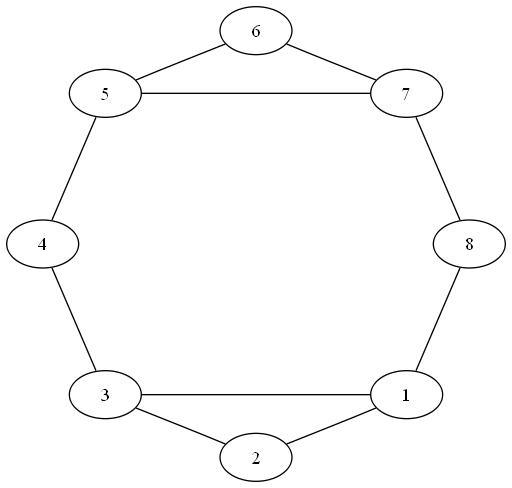
\includegraphics[width=0.5\linewidth]{./graph2.jpg}
	%%\caption{}
	%\label{fig:graph2}
	%\end{figure}
	\item State the vertices that comprise a cycle of length 5 in both of the following graphs.
	%\begin{figure}[h!]
	%\centering
	%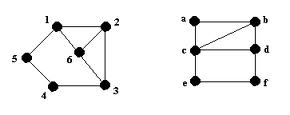
\includegraphics[width=0.7\linewidth]{./graph20.jpg}
	%
	%\label{fig:graph20}
	%\end{figure}
\end{enumerate}








%------------------------------------%

\section*{Session 05 Graph Theory}
\begin{itemize}
	\item Eulerian Path
	\item Isomorphism
	\item Adjacency matrices
\end{itemize}
Adjacency Matrices
\[ \left( \begin{matrix}
o & 1 & 0 & 1 & 1 \\ 
1 & 0 & 1 & 0 & 1 \\ 
1 & 1 & 0 & 1 & 1 \\ 
0 & 1 & 1 & 1 & 1 \\ 
1 & 1 & 0 & 1 & 0
\end{matrix} \right) \]


\section*{Session 05 Graph Theory}
\begin{itemize}
	\item Eulerian Path
	\item Isomorphism
	\item Adjacency matrices
\end{itemize}
Adjacency Matrices
\[ \left( \begin{matrix}
o & 1 & 0 & 1 & 1 \\ 
1 & 0 & 1 & 0 & 1 \\ 
1 & 1 & 0 & 1 & 1 \\ 
0 & 1 & 1 & 1 & 1 \\ 
1 & 1 & 0 & 1 & 0
\end{matrix} \right) \]

\section{graph theory }
Given the following definitions for simple, connected graphs:
\begin{itemize}
	\item $K_n$ is a graph on $n$ vertices where each pair of vertices is connected by an edge;
	\item $C_n$ is the graph with vertices $v_1, v_2, v_3, \dots, v_n$ and edges $\{v_1,v_2\}, \{v_2,v_3\}, \dots\{v_n, v_1\}$;
	\item $W_n$ is the graph obtained from $C_n$ by adding an extra vertex,$v_{n+1}$, and edges
	from this to each of the original vertices in $C_n$.
\end{itemize}
(a) Draw $K_4$, $C_4$, and $W_4$. 
%----------------------------------------------------------------%
\newpage
\section*{Condtions for Isomorphism}
\begin{itemize}
	\item
	\item
	\item
\end{itemize}

%--------------------------- %
% Section 6 Digraphs and Relations
\section*{Question 6}
%Relations and Digraphs

%------------------------------------%
\chapter{Session 6}
\section*{Session 06: Digraphs and Relations}
\begin{itemize}
	\item[6A.1] In-degree and out-degree
	\item[6A.2]
	\item[6A.3]
\end{itemize}
\subsection*{Relations}
\begin{itemize}
	\item[6B.1] Equivalence RElations (6.2.2)
	\item[6B.2]
	\item[6B.3] Relations and Cartesian Products (6.3)
\end{itemize}


\begin{itemize}
	\item \textbf{Reflexive}: 
	\item \textbf{Symmetric}: 
	\item \textbf{Transitive}: 
	\item \textbf{Anti-symmetric}: 
	\item \textbf{Equivalence Relation}: 
	\item \textbf{Partial Order}:
	\item \textbf{Order}:
\end{itemize}

%-----------------------------------------------------%
\section*{Question 6}

\subsection*{Part A : Digraphs}

Suppose $A = \{1,2,3,4\}$. Consider the following relation in A

\[ \{  (1,1),(2,2),(2,3),(3,2),(4,2),(4,4)\} \]

Draw the direct graph of $A$. Based on the Digraph of $A$ discuss whether or not a relation that could be depicted by the digraph could be described as the following, justifying your answer.


\begin{itemize}
	\item[(i)] Symmetric
	\item[(ii)] Reflexive 
	\item[(iii)] Transitive
	\item[(iv)] Antisymmetric
\end{itemize}
\subsection*{Part B : Relations}
Determine which of the following relations $ x R y$ are reflexive, transitive, symmetric, or antisymmetric on the following - there may be more than one characteristic.  if

\begin{itemize} 
	\item[(i)] $x = y$
	\item[(ii)] $x < y$
	\item[(iii)] $x^2 = y^2$
	\item[(iv)] $x \geq y$
\end{itemize}
\subsection*{Part C : Partial Orders}
% http://staff.scem.uws.edu.au/cgi-bin/cgiwrap/zhuhan/dmath/dm_readall.cgi?page=20

Let $A=\{0,1,2\}$ and $R=\{ (0,0),(0,1),(0,2),(1,1), (1,2), (2,2)\}$
and $S=\{(0,0),(1,1),(2,2)\}$ be 2 relations on A. Show that

\begin{itemize}
	\item[(i)] R is a partial order relation.
	\item[(ii)] S is an equivalence relation.
\end{itemize}



\section{Digraphs and Relatiosn}
% 2007 Q8
Given a flock of chickens, between any two chickens one of them is
dominant. A relation, R, is defined between chicken x and chicken y as xRy if x is
dominant over y. This gives what is known as a pecking order to the flock. Home
Farm has 5 chickens: Amy, Beth, Carol, Daisy and Eve, with the following relations:

\begin{itemize}
	\item Amy is dominant over Beth and Carol
	\item Beth is dominant over Eve and Carol
	\item Carol is dominant over Eve and Daisy
	\item Daisy is dominant over Eve, Amy and Beth
	\item Eve is dominant over Amy.
\end{itemize}

\newpage

\chapter{Session 7}
	
	%------------------------------------%
	
				\section*{Session 07:Sequences and Series}
				\begin{itemize}
					\item[7A.1] Sequences
					\item[7A.2] Induction
					\item[7A.3] Series and the Sigma Notation
				\end{itemize}
				
				\subsection*{Recurrence Relations(7.1.1)}
				
				
				
				$u_1 = 2$
				$u_2 = u_1 + 3 = 2 +3 = 5$
				$u_3 = u_2 + 3 = 5+ 3 = 8$
				Airthmetic Progression
				
				
				\subsection*{Proof by Induction(7.2.2)}
				\begin{itemize}
					\item[Step 1] Base case
					\item[Step 2] Induction hypothesis
					\item[Step 3] Induction step
				\end{itemize}
				
				
				
				\subsection*{Series and Sigma Notation(7.2.3)}
				
				
				%-----------------------------------------------------%
				
	\section*{Question 7}
	\subsection*{Part A : Recurrence Relations}
	A sequence is defined by the recurrence relations
	\[x_{n+2}  = 3x_{n+1} - 2x_n\]
	with initial terms $x_1 = 1$ and $x_2=3$.
	
	\begin{itemize}
		\item[(i)] Calculate $x_3$, $x_4$ and $x_5$, showing your workings.
		\item[(ii)] Prove by induction that $x_n = 2^n - 1$ for all $n \geq 1$
	\end{itemize}
	
	%------------------------------------%
	\subsection*{Part B : Summations}
	
	Compute the following summation
	
	\[ \sum^{i=100}_{i=25} i^2 + 3i -5)\]
	%------------------------------------%
	
	
	Say which of the set the following numbers belong to.
	
	If they belong to more than one of these sets, give all the sets.
	
	$\sqrt{2}$
	$\frac{3}{7}$
	
	%------------------------------------------------------
	
	
	
	\subsection*{Section 8 Exercises}
	\begin{itemize}
		\item $8^{\frac{1}{3}}$ Recall $a^{\frac{b}{c}} = a^{\frac{b}{c}}$
		\item
		\item
	\end{itemize}
	
	
	
	
	%------------------------------------%
	
	\section*{Question 7b}
	
	Compute the following summation
	
	\[ \sum^{i=100}_{i=25} i^2 + 3i -5)\]
	
	
	%------------------------------------%
	
\section*{Question 7}
\subsection{Question 7a}

A sequence is defined by the formula 
$u_n = 5n-3$ for $n\geq 1$

\[\frac{n(n+1)(2n+1)}{6}\]

Write the following sums in the $\Sigma$ notation and evaluate them

\begin{itemize}
	\item $1^2 + 2^2 + 3^2 +  \ldots +  40^2 = ?$
	\item $2 + 5 + 10 + \ldots + 1601 = ?$
	\item $2+8+18+\ldots +3200 = ?$
\end{itemize}

\subsection*{Part A : Recurrence Relations}
A sequence is defined by the recurrence relations
\[x_{n+2}  = 3x_{n+1} - 2x_n\]
with initial terms $x_1 = 1$ and $x_2=3$.

\begin{itemize}
	\item[(i)] Calculate $x_3$, $x_4$ and $x_5$, showing your workings.
	\item[(ii)] Prove by induction that $x_n = 2^n - 1$ for all $n \geq 1$
\end{itemize}

%------------------------------------%




\section*{Proof By Induction}

\begin{itemize}
	\item \textbf{Base Step}
	\item \textbf{Induction Step}
	\item \textbf{Some Step}
\end{itemize}

%------------------------- %
%-------------------------- %

%------------------------------------%
\subsection{Sequence and Series and Proof by Induction}


\[\sum^{n}_{i=1} (n^2) \]

\chapter{Session 8}
% % Section 8 Trees
	%-----------------------------------------------------%
	\section*{Question 8}
	\subsection*{Part A : Spanning Trees}
	\begin{enumerate}
		\item How many edges are in the spanning tree $T$ ?
		\item What is the sum of the degree sequence of $T$?
		\item Write down all the possible degree sequences for the spanning tree $T$.
	\end{enumerate}
	%------------------------------------%
	
	\subsection*{Part B : Binary Search Trees}
	Suppose a database, comprised of 30,000 internal nodes, is structured as a Binary Search Tree.
	
	\begin{enumerate}
		\item What is the key (number) of the Root node?
		\item What are the keys of the nodes at level 1?
		\item For the nodes at level1, how many subtrees are there?
		\item State which nodes are in the substrees of the level 1 nodes?
		\item How many nodes are the between the root (level 0) and level 7. ]
		(Hint: use a summation theorem mentioned in session 7
		\item What is the maximum number of searchs in this database?
	\end{enumerate}
	
	
	
	
	\section{Question 8B}
	Suppose a database, comprised of 30,000 internal nodes, is structured as a Binary Search Tree.
	
	\begin{enumerate}
		\item What is the Key of the Root node?
		\item What are the keys of the nodes at level 1?
		\item For the nodes at level1, how many subtrees are there?
		\item State which nodes are in the substrees of the level 1 nodes?
		\item How many nodes are the between the root (level 0) and level 7. ]
		(Hint: use a summation theorem mentioned in session 7
		\item What is the maximum number of searchs in this database?
	\end{enumerate}
	%--------------------------------------------------------------------
	
\section*{Binary Search Trees}
What is a Binary Search Tree
\[ \lfloor  \frac{\mbox{log}_2}{T} \rfloor \]

%------------------------- %
%-------------------------- %
				\section*{Session 08:Trees}
				\begin{itemize}
					\item[8A.1] Trees
					\item[8A.2] Spanning Trees
					\item[8A.3] Rooted trees
					\item[8A.4] Binary Search Trees
				\end{itemize}
				A tree is a directed graph that contains no cycles.
				%-----------------------------------------------------%
\section{Question 8}

1) Draw this tree
2) Construct all the isomorphic tress with 6 vertices which can be obtainbed by attaching a new vertex of degreee one to a vertex of T.
3) Explain briefly why the tree obtained in (ii) is not isomorphic to each other.
4) Construct a tree with 6 vertices which is not isomorphic to any tree you constructed in (ii)

Part b
Determine the number of nodes on level 5 and level 10
Find an expression in terms of $\Sigma$ and h for the number of internal nodes in such a tree.
What is the smallest possible height of such a tree if there are at least 900 internal nodes.

% %------------------------------------------------------

\section{Question 8A}
\begin{enumerate}
	\item How many edges are in the spanning tree $T$ ?
	\item What is the sum of the degree sequence of $T$?
	\item Write down all the possible degree sequences for the spanning tree $T$.
\end{enumerate}
%------------------------------------%
\chapter{Session 9}
\section{Probability and Counting}

% 2007 Q8
Given S is the set of all 5 digit binary strings, E is the set of a 5 digit
binary strings beginning with a 1 and F is the set of all 5 digit binary strings ending
with two zeroes.
\begin{itemize}
	\item[(a)] Find the cardinality of S, E and F.
	\item[(b)] Draw a Venn diagram to show the relationship between the sets S, E and F.
	\item[(c)]Show the relevant number of elements in each region of your diagram.
\end{itemize}
%-------------------------------------------------------------------------%
\newpage




%------------------------- %
% Section 1
\subsection{Axioms of Probability}

The Axioms of Probability

\begin{itemize}
	\item The probability of a certain event is 1.
	\item The probability of an impossible event is 0.
	\item 
\end{itemize}
%------------------------- %
%-------------------------- %
				\section*{Session 09: Probability}
				\begin{itemize}
					\item[9A.1] Counting Methods
					\item[9A.2] Counting using Sets
					\item[9A.3] Probability
					\item[9A.4] Independent Events
				\end{itemize}
				\begin{itemize}
					\item[9B.1] Permutation
					
					\[ {n \choose r} = \frac{n!}{(n-r)! r!} \]
					
					
					\[ {6 \choose 3} = \frac{6!}{(6-3)! 3!} = \frac{6!}{3! \times 3!}\]
					
					
					\[ \frac{6!}{3! \times 3!} = \frac{6 \times 5 \times 4 \times 3!}{3! \times 3!} = \frac{120}{6} = 120\]
				\end{itemize}
				%		\begin{multicol}{2}
				\begin{itemize}
					\item ${6 \choose 2} = 15$
					\item ${5 \choose 2} = 10$  
					\item ${4 \choose 0} = 1$  
					\item ${4 \choose 3} = 4$  
				\end{itemize}
				%		\end{multicol}
				
				\begin{itemize}
					\item pairwise disjoint sets
					\item The addition principle
				\end{itemize}
				\subsection*{Theorem}
				\[ |A \cup B| = |A| + |B| - |A \cap B|  \]
				
				\subsection*{Probability}
				\begin{itemize}
					\item[9B.2] The sample space of an experiment ($S$)
					\item[9B.3] The size of a sample space
					\item[9B.4] Indepedent Evcents (9.3.1)
				\end{itemize}
				%-----------------------------------------------------%
				

%------------------------------------------------%
\section*{Session 9 Probability}
\subsection*{Binomial Coefficients}
\begin{itemize}
	\item factorials 
	\[ n! = (n)\times (n-1)\times(n-2) \times \ldots \times 1 \]
	\begin{itemize}
		\item $5! = 5 \times 4 \times 3 \times 2 \times 1 = 120 $
		\item $3! = 3 \times 2 \times 1$
	\end{itemize}
	\item Zero factorial
	\[ 0! =  1 \]
\end{itemize}
%---------------------------------------------- %

% \[P(A |B = \frac{P(A \cap B)}{P(B)})\]

The complement rule in Probability

$P(C^{\prime}) = 1- P(C)$



If the probability of C is $70 \%$ then the probability of $C^{\prime}$ is $30\%$


%------------------------------------------------%
\section*{Probability}
\subsection*{Binomial Coefficients}
\begin{itemize}
	\item factorials 
	\[ n! = (n)\times (n-1)\times(n-2) \times \ldots \times 1 \]
	\begin{itemize}
		\item $5! = 5 \times 4 \times 3 \times 2 \times 1 = 120 $
		\item $3! = 3 \times 2 \times 1$
	\end{itemize}
	\item Zero factorial
	\[ 0! =  1 \]
\end{itemize}
%---------------------------------------------- %

% \[P(A |B = \frac{P(A \cap B)}{P(B)})\]

The complement rule in Probability

$P(C^{\prime}) = 1- P(C)$



If the probability of C is $70 \%$ then the probability of $C^{\prime}$ is $30\%$


\section{Counting}
% 2007 Q8
Given S is the set of all 5 digit binary strings, E is the set of a 5 digit
binary strings beginning with a 1 and F is the set of all 5 digit binary strings ending
with two zeroes.
\begin{itemize}
	\item[(a)] Find the cardinality of S, E and F.
	\item[(b)] Draw a Venn diagram to show the relationship between the sets S, E and F.
	\item[(c)] Show the relevant number of elements in each region of your diagram.
\end{itemize}

\section*{Probability: Binomial Coefficients}
\begin{itemize}
	\item factorials 
	\[ n! = (n)\times (n-1)\times(n-2) \times \ldots \times 1 \]
	\begin{itemize}
		\item $5! = 5 \times 4 \times 3 \times 2 \times 1 = 120 $
		\item $3! = 3 \times 2 \times 1$
	\end{itemize}
	\item Zero factorial
	\[ 0! =  1 \]
\end{itemize}
%---------------------------------------------- %

% \[P(A |B = \frac{P(A \cap B)}{P(B)})\]

The complement rule in Probability

$P(C^{\prime}) = 1- P(C)$



If the probability of C is $70 \%$ then the probability of $C^{\prime}$ is $30\%$
\chapter{Session 10 }
Systems of Linear Equation
\section{Matrices}

What are the dimensions of the following matrix


\[ \left(
\begin{array}{cc}
a_1 & a_2 \\ 
b_1 & b_2
\end{array} \right)\left(
\begin{array}{cc}
c_1 & d_1 \\ 
c_2 & d_2
\end{array} \right) = \left(
\begin{array}{cc}
(a_1 \times c_1) + (a_2 \times c_2) & (a_1 \times d_1) + (a_2 \times d_2) \\ 
(b_1 \times c_1) + (b_2 \times c_2) & (b_1 \times d_1) + (b_2 \times d_2)
\end{array} \right) \]

\bigskip
\large{
	\[ \left(
	\begin{array}{cc}
	1 & 3 \\ 
	0 & 2
	\end{array} \right)\left(
	\begin{array}{cc}
	1 & 2 \\ 
	4 & 1
	\end{array} \right) = \left(
	\begin{array}{cc}
	(1 \times 1) + (3 \times 4) & (1 \times 2) + (3 \times 1) \\ 
	(0 \times 4) + (2 \times 4) & (0 \times 2) + (2 \times 1)
	\end{array} \right) = \left(
	\begin{array}{cc}
	14 & 5 \\ 
	8 & 2
	\end{array} \right) \]
}

\[ \left(
\left(
\begin{array}{cc}
1 & 2 \\ 
4 & 1
\end{array} \right)
\begin{array}{cc}
1 & 3 \\ 
0 & 2
\end{array} \right) = ? \]



\section*{Reduced Echelon Form}

\begin{itemize}
	\item
	\item
	\item
\end{itemize}


					\section*{Session 10: Matrices and Systems of Equations}
					\begin{itemize}
						\item[10A.1] Dimensions of a Matrix
						\item[10A.2] Matrix Multiplication
						\item[10A.3] Matrix Calculations
						\item[10A.4] 
					\end{itemize}
					
					\begin{itemize}
						\item[10B.1] Systems of Equations
						\item[10B.2] Expression Systems of Equations as Matrices
						\item[10B.3] Augmented Matrices
						\item[10B.4] Guassian Elimination
					\end{itemize}
					
					
					%-----------------------------------------------------%
					
					
					
					
					
					
					
					
					
					
					
					
					
					
					%-----------------------------------------------------%
					
					
					
\section*{Question 10}

\subsection*{Session 10: Matrices and Systems of Equations}
\begin{itemize}
	\item[10A.1] Dimensions of a Matrix
	\item[10A.2] Matrix Multiplication
	\item[10A.3] Matrix Calculations
	\item[10A.4] 
\end{itemize}

\begin{itemize}
	\item[10B.1] Systems of Equations
	\item[10B.2] Expression Systems of Equations as Matrices
	\item[10B.3] Augmented Matrices
	\item[10B.4] Guassian Elimination
\end{itemize}
%-----------------------------------%
\subsection*{Question 10A}

Say what information the first row of the matrix contains.
Find the number of edges of G.


Write doen the augmented matrix for the following system of equations.
x+y+2z=7
2x+y+3z =11
x-27+5z=4


Use Gaussian elimination to solve the system.

\subsection*{Part B : Summations}

Compute the following summation

\[ \sum^{i=100}_{i=25} i^2 + 3i -5)\]

\section{Matrices}

What are the dimensions of the following matrix


\[ \left(
\begin{array}{cc}
a_1 & a_2 \\ 
b_1 & b_2
\end{array} \right)\left(
\begin{array}{cc}
c_1 & d_1 \\ 
c_2 & d_2
\end{array} \right) = \left(
\begin{array}{cc}
(a_1 \times c_1) + (a_2 \times c_2) & (a_1 \times d_1) + (a_2 \times d_2) \\ 
(b_1 \times c_1) + (b_2 \times c_2) & (b_1 \times d_1) + (b_2 \times d_2)
\end{array} \right) \]

\bigskip
\large{
	\[ \left(
	\begin{array}{cc}
	1 & 3 \\ 
	0 & 2
	\end{array} \right)\left(
	\begin{array}{cc}
	1 & 2 \\ 
	4 & 1
	\end{array} \right) = \left(
	\begin{array}{cc}
	(1 \times 1) + (3 \times 4) & (1 \times 2) + (3 \times 1) \\ 
	(0 \times 4) + (2 \times 4) & (0 \times 2) + (2 \times 1)
	\end{array} \right) = \left(
	\begin{array}{cc}
	14 & 5 \\ 
	8 & 2
	\end{array} \right) \]
}

\[ \left(
\left(
\begin{array}{cc}
1 & 2 \\ 
4 & 1
\end{array} \right)
\begin{array}{cc}
1 & 3 \\ 
0 & 2
\end{array} \right) = ? \]


%---------------------------------------%
\subsection*{Question 1}

\begin{enumerate}[(i)]
	\item (1 Mark) When is the positive integer $p$ said to be a prime number?
	\item (2 Marks) Express the following hexadecimal number as a decimal number, and as a binary number: \[(A32.8)_{16}\]
	
	\item (2 Marks) Convert the following decimal number into base 2, showing all your working:
	$(253)_{10}$. 
	\item (2 Marks) Covert the decimal integer $(407)_{10}$ to binary notation.
	
	\item (2 Marks) Showing your working, express the following number 
	\[ 1.024024024024\ldots\]
	as a ration number in its simplest form.
	\item (1 Mark) Compute the following $101101_2 + 1101_2$ 
\end{enumerate}
%--------------------------------------------------- %
\subsection*{Question 2}
%Question 2
Let A and B and C be subsets of a universal set U.
\begin{itemize}
	\item[(a)] (1 Mark) Draw a labelled Venn diagram depicting A,B,C in such a way that they divide
	U into 8 disjoint regions. [1]
	\item[(b)] (3 Marks) The subset $X \subseteq U$ is defined by the following membership table below. Shade the region X on your diagram. Describe the region you have shaded in
	set notation as simply as you can. 
\end{itemize}
{\LARGE
	\begin{center}
		\begin{tabular}{|c|c|c|c|}
			\hline
			A & B & C & X \\ \hline
			0 & 0 & 0 & 0 \\ \hline
			0 & 0 & 1 & 1 \\ \hline
			0 & 1 & 0 & 0 \\ \hline
			0 & 1 & 1 & 0 \\ \hline
			1 & 0 & 0 & 1 \\ \hline
			1 & 0 & 1 & 1 \\ \hline
			1 & 1 & 0 & 1 \\ \hline
			1 & 1 & 1 & 0 \\ \hline
		\end{tabular} 
	\end{center}
}
\begin{itemize}
	\item[(c)] (3 Marks) The subset $Y \subseteq U$ is defined as $Y = A \cup (C - B)$. Construct the membership
	table for Y. 
	\item[(d)] (3 Marks) For each of the following statements say whether it is true or false, justifying
	your answer, using the Venn diagram you drew earlier.
	
	\begin{enumerate}[(i)]
		\item $Y \subseteq X$
		\item $Y^{\prime} \subseteq X^{\prime}$
		\item $Y - X = A \cap B \cap C$.
	\end{enumerate}
\end{itemize}
%=====================================================================%
\subsection*{Question 3}
%2003

\begin{itemize}
	\item[(a)] Let n be an element of the set $\{10, 11, 12, 13, 14, 15, 16, 17, 18, 19\}$,
	and p and q be the propositions:
	\[p : n \mbox{ is odd},   q : n < 15\]. Draw up truth tables for the following statements and find the values of n for
	which they are true:
	\begin{itemize}
		\item[(i)] $ p \vee \neg q$ 
		\item[(ii)] $\neg p \wedge q$
	\end{itemize}
	\item[(b)] Use truth tables to find a statement that is logically equivalent to $\neg p \rightarrow q$.
\end{itemize}

%--------------------- %
% - 1.2 2010 
\begin{enumerate}[(i)]
	\item
\end{enumerate}
%=====================================================================%
\subsection*{Question 4}
Let $S$ be the set of all 4 bit binary strings. The function $f : S \rightarrow Z$
is defined by the rule:
\[f(x) = \mbox{ the number of zeros in x} \] for each binary string $x \in S$.
Find:
\begin{itemize}
	\item[(a)] (4 Marks) Answer the following questions
	\begin{itemize}
		\item[(i)] the number of elements in the domain
		\item[(ii)] f(1010)
		\item[(iii)] the set of pre-images of 1
		\item[(iv)] the range of f. 
	\end{itemize}
	\item[(b)] (2 Marks) Decide whether the function $f$, as defined above, has either the one to one or
	the onto property, justifying your answers. 
	\item[(c)] (2 Marks) State the condition to be satisfied by a function $f : X \rightarrow Y$ for it to have an
	inverse function $f^{-1} : Y \rightarrow X$.
	\item[(d)] (2 Marks) Define the inverse functions for each of the following:
\end{itemize}
%---------------------------------------------------------%
%\section*{Question 5}
%
%\begin{figure}
%	\centering
%	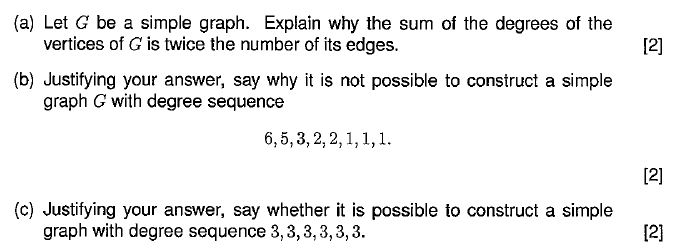
\includegraphics[width=0.7\linewidth]{GraphTheoryQuestion2012}
%	
%\end{figure}

\section*{Question 5}
Given the following definitions for simple, connected graphs:
\begin{itemize}
	\item $K_n$ is a graph on $n$ vertices where each pair of vertices is connected by an edge;
	\item $C_n$ is the graph with vertices $v_1, v_2, v_3, \dots, v_n$ and edges $\{v_1,v_2\}, \{v_2,v_3\}, \dots\{v_n, v_1\}$;
	\item $W_n$ is the graph obtained from $C_n$ by adding an extra vertex,$v_{n+1}$, and edges
	from this to each of the original vertices in $C_n$.
\end{itemize}
(a) Draw $K_4$, $C_4$, and $W_4$. 

%----------------------------- %
% 2006 
a) (i) A simple, connected graph has 7 vertices, all having the same degree d.
State the possible values of d and for each value also give the number of edges
in the corresponding graph.
(ii) Another simple, connected graph has 6 vertices, all having the same degree,
n. Draw such a graph when n = 3 and state the other possible values of n.
[4]
%----------------------------------------------------------------%
\newpage
\section*{Question 6}
% 2007 Q8
Given a flock of chickens, between any two chickens one of them is
dominant. A relation, R, is defined between chicken x and chicken y as xRy if x is
dominant over y. This gives what is known as a pecking order to the flock. Home
Farm has 5 chickens: Amy, Beth, Carol, Daisy and Eve, with the following relations:

\begin{itemize}
	\item Amy is dominant over Beth and Carol
	\item Beth is dominant over Eve and Carol
	\item Carol is dominant over Eve and Daisy
	\item Daisy is dominant over Eve, Amy and Beth
	\item Eve is dominant over Amy.
\end{itemize}

\newpage
\section*{Question 6}
% Digraphs and Relations
% http://staff.scem.uws.edu.au/cgi-bin/cgiwrap/zhuhan/dmath/dm_readall.cgi?page=20

Let $A=\{0,1,2\}$ and $R=\{ (0,0),(0,1),(0,2),(1,1), (1,2), (2,2)\}$
and $S=\{(0,0),(1,1),(2,2)\}$ be 2 relations on A. Show that

\begin{itemize}
	\item[(i)] R is a partial order relation.
	\item[(ii)] S is an equivalence relation.
\end{itemize}
%---------------------------------------------------------------------------%

%2002 Question 7
Let S be a set and let R be a relation on S
Explain what it means to say thet $\mathcal{R}$ is

\begin{itemize}
	\item[(i)] reflexive
	\item[(ii)] symmetrix
	\item[(iii)] anti-symmetric
	\item[(iv)] Transitive
	%---------------------------------------------------------------------------%
	
	
	
\end{itemize}


%--------------------------------------------------------------------------- %
\section*{Question 7}
Let the sequence un be defined by the recurrence relation
\[u_{n+1} = u_n + 2n, \mbox{ for n = 1, 2, 3, ...}\]
and let $u_1 = 1$.\\
%\begin{figure}[h!]
%	\centering
%	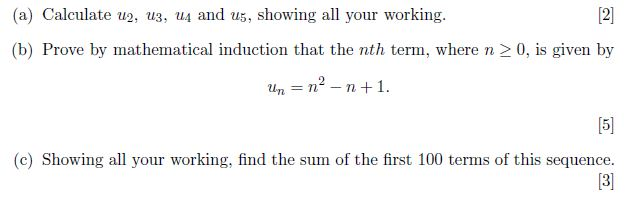
\includegraphics[width=1.11\linewidth]{SeqSerQuestion2005}
%\end{figure}

%---------------------------------------------------------------------------%
% TREES
\newpage
\section*{Question 8}
%\noindent \textbf{(Part A : Spanning Trees -  5 Marks) }\\
%\begin{figure}[h!]
%	\centering
%	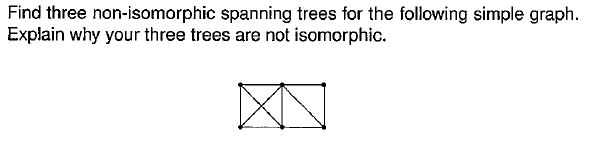
\includegraphics[width=1.11\linewidth]{TreesQuestion2012}
%\end{figure}

%	Question 8A
%	\begin{enumerate}
%		\item How many edges are in the spanning tree $T$ ?
%		\item What is the sum of the degree sequence of $T$?
%		\item Write down all the possible degree sequences for the spanning tree $T$.
%	\end{enumerate}
%---------------------------------------------------------------------------%


\noindent \textbf{(Part B :Binary Search Trees -  5 Marks) }\\
Suppose a database, comprised of 30,000 internal nodes, is structured as a Binary Search Tree.

\begin{enumerate}[(i)]
	\item What is the Key of the Root node?
	\item What are the keys of the nodes at level 1?
	\item For the nodes at level 1, how many subtrees are there?
	%	\item State which nodes are in the substrees of the level 1 nodes?
	\item How many nodes are the between the root (level 0) and level 4. ]
	%	(Hint: use a summation theorem mentioned in session 7
	\item What is the maximum number of searchs in this database?
\end{enumerate}

%============================================================================%

\section*{ Question 9 }
Given S is the set of all 5 digit binary strings, E is the set of a 5 digit
binary strings beginning with a 1 and F is the set of all 5 digit binary strings ending
with two zeroes.
\begin{itemize}
	\item[(a)] Find the cardinality of S, E and F.
	\item[(b)] Draw a Venn diagram to show the relationship between the sets S, E and F.
	Show the relevant number of elements in each region of your diagram.
\end{itemize}

\begin{itemize}
	\item A college teaches courses in the following subjects areas: mathematics, computing and statistics.
	\item Students in the college may choose their courses from these three subject areas.
	\item Students are not obliged to take courses from these three subject areas, and may instead take courses in other subject areas. 
	\item  Let the subject areas be represented by the letters \textbf{M} for mathematics, \textbf{C} for computing and \textbf{S} for statistics. \item Draw a labelled Venn diagram showing the areas \textbf{M}, \textbf{C}, and \textbf{S} in such a way as to represent the students studying at the college. \item On your diagram show the number of students studying in each region of the Venn diagram.
	%===================%
	\begin{itemize}
		\item Currently 600
		students are enrolled in the college. 
		\item 300 students are taking mathematics courses.
		\item 120 student are taking statistics courses.
		\item 380 students are taking computing courses. 
		\item 40 students study courses from all three subject
		areas. 
		\item 200 mathematics students are taking computing courses as well. \item 60 computing students
		are also takings statistics courses. \item  70 statistics students are also taking mathematics course.
	\end{itemize}
\end{itemize}

%==============%
\begin{itemize}
	\item[(i)] How many students study none of these courses at all?
	\item[(ii)] How many students are taking mathematics courses but not computing or statistics courses.
	\item[(iii)] How many students study courses from precisely two of these subject
	areas?
	
\end{itemize}
\newpage
%===========================================================%
\section*{Question 10}
%%--------------------------------------------%
%\noindent \textbf{Part A : Matrix Operations - 4 Marks}\\ 
%\begin{figure}[h!]
%	\centering
%	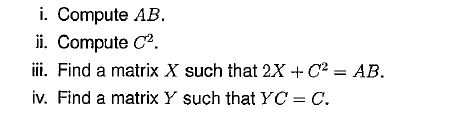
\includegraphics[width=1.11\linewidth]{MatrixQuestion2012}
%	
%\end{figure}


%--------------------------------------------%
\noindent \textbf{Part B : Gaussian Elimination - 5 Marks}\\ 
\begin{itemize}
	\item[(i)] Say whether or not the graphs they represent are isomorphic.
	\item[(ii)] Calculate $A^2$ and $A^4$ and say what information each gives about the graph
	corresponding to A. [6]
\end{itemize}
%===========================================%
\begin{itemize}
	\item[(i)] Write down the augmented matrix for the following system of equations.
	\[2x + y - z = 2\]
	\[x - y + z = 4\]
	\[x + 2y + 2z = 10\]
	\item[(ii)] Use Gaussian elimination to solve the system. 
\end{itemize}
%=========================================================================================== %


%-------------------------------------------------------------------------%
\newpage

\end{document}